\chapter{Evaluation} % Main chapter title

\label{Chapter5} % For referencing the chapter elsewhere, use \ref{Chapter1} 

\lhead{Chapter 5. \emph{Evaluation}}
This chapter evaluates the approach presented in Chapter \ref{Chapter3} to answer the proposed research questions. Section \ref{evalsetup} introduces the candidates selected for the empirical evaluation and describes the experimental setup. Section \ref{expeval} presents the results of the experimental evaluation.  

\section{Experimental Setup}
\label{evalsetup}
For the evaluation of the proposed approach, our goal was to select candidates that satisfy the project requirements described in Section \ref{selectingCandidates}. Unfortunately, not many applications which satisfy the aforementioned requirements are available and have publicly accessible Selenium test suites. In order to evaluate the research questions, five commercial-scale open-source web applications as described in Table \ref{appcandidates} have been selected. All of these applications have several years of software development history.

Among the experimental candidates, Moodle\footnote{\url{https://moodle.org/}} is a widely used open-source Course Management System. Mozilla Addons\footnote{\url{https://addons.mozilla.org/}} web application hosts web-browser extensions. Mozilla Marketplace\footnote{\url{https://marketplace.firefox.com/}} is an online app portal for desktop and mobile platforms, while Mozilla.org\footnote{\url{https://www.mozilla.org/}} serves as the home for the Mozilla project. Our last candidate, Jenkins\footnote{\url{https://jenkins-ci.org/}}, is a popular open-source continuous integration tool. 
  
Each of these applications is installed as per the automated deployment process explained in Section \ref{sec:autoDeployment}. The automated deployment process also ensures that the AUT is always installed to a `clean' state. As mentioned in Chapter \ref{Chapter4}, our approach considers different major and minor versions of candidate web applications. This setup allows us to evaluate the incremental changes to the AUT in the form of minor revisions of different major releases. 
Since different applications have different development and release cycles, we have considered approximately one year of development time-frame for each application. 

  \begin{table}
  \centering
  \resizebox{14.3cm}{!}{
  \begin{tabular}{l*{6}{l}r}
  % \\ 
  \hline
  Application              & Domain &  Major Versions & Minor Versions \\
  \hline
  Moodle            & Course Management System & 1 & 11  \\
  Marketplace     & Software Apps portal  & 4 & 22   \\
  Addons           & Browser Add-ons portal & 3 & 20  \\
  Mozilla.org     & Mozilla Project Homepage & 2 & 18   \\
  Jenkins (LTS/ Weekly) & Continuous Integration tool & 4/ 4 & 12/ 23   \\
  % Jenkins  & Continuous Integration tool & 4 & 23  \\
  \hline
  \end{tabular}}
   \captionsetup{justification=justified,
singlelinecheck=false}
  \caption{Overview of evaluation candidate web applications. `Major Versions' indicate total number of major releases. `Minor version' represents total number of minor revisions. (Note: For Jenkins, two release cycles -- Long Term Support (LTS) and Weekly releases are considered.) }
  \label{appcandidates}
  \end{table}

The approach illustrated in Section \ref{selectingCandidates} has been followed for selecting the major and minor releases of candidate web applications. Out of the selected web applications, only Moodle classifies the releases in terms of major-minor versions. All of the other applications do not identify their releases in this manner. Mozilla Addons and Marketplace follow weekly release cycles. Mozilla.org does not adhere to any specific release cycle and delivers important features and bug fixes by pushing necessary commits to its version control repository. Jenkins has two different release cycles -- Long Term Support (LTS) and weekly releases. The weekly cycle releases a new Jenkins version on weekly basis and frequently introduces new features as well as bug fixes. The LTS cycle, on the other hand, has relatively fewer but more stable monthly releases. Both of these release lines have been considered for the evaluation, since it would be interesting to compare how the development process of the AUT affect the results. The chosen major and minor versions for all candidate web applications are listed in Appendix \ref{AppendixA}.

Table \ref{testcandidates} gives an overview about the test-suites of these open-source web applications. Each test-suite repository has several hundreds of commits from various contributors. The instructions for running these test-suites are also provided by the respective organizations. All of the selected web applications follow the page-object pattern for developing their Selenium test-suites. While Jenkins\footnote{\url{https://github.com/jenkinsci/acceptance-test-harness}} and Moodle\footnote{\url{https://git.in.moodle.com/tomb/functional-test-suite}} test-suites are primarily written in Java, the Mozilla Addons\footnote{\url{https://github.com/mozilla/Addon-Tests}}, Marketplace{\footnote{\url{https://github.com/mozilla/marketplace-tests}}} and Mozilla.org\footnote{\url{https://github.com/mozilla/mcom-tests}} test-suites are written in Python.
Excluding Moodle, all other test-suites have been maintained in parallel to the development of chosen web application revisions 
% for the entire duration of the experimental phase of this thesis 
(as of March 2016, Moodle and Mozilla.org test-suite repositories have been archived and are no longer actively maintained). The `Size' column in Table \ref{testcandidates} indicates the average number of tests per test-suite. Apart from Mozilla Marketplace, all other test-suites have fairly comparable sizes. For Moodle test-suite, 38 out of 45 tests are parameterized. A parameterized test denotes a test case executed with different input values. 
\begin{table}
\centering
\resizebox{8.5cm}{!}{
\begin{tabular}{l*{6}{l}r}
\hline
Test-Suite              & Language & Page-objects & Size &LOC \\
\hline
Moodle           & Java & 13 & 43 & 2103  \\
Marketplace     & Python & 12 & 10 & 981
 \\
Addons           & Python & 17  & 55 & 3335
 \\
Mozilla.org    & Python & 16 & 60 & 2419 \\
Jenkins  & Java & 35 & 52 & 8755  \\
\hline
\end{tabular}}
\caption{Overview of Selenium test-suites for candidate web applications}
\label{testcandidates}
\end{table}

We selected these tests by executing the test-suite for the major versions of each application over multiple runs and identifying the number of ``passed'' tests, as per the approach described in Section \ref{selectingCandidates}. As a consequence, these ``passed'' tests represent a subset of the total number of available tests from the chosen candidate test-suites. The reason for selecting this subset is that the tests which were marked as ``failed'' were not suitable to be considered for the robustness analysis, as they did not cover the intended functionality for the major versions in the first place. 
% There could be myriad of reasons behind this behavior, which have been briefly mentioned in Section \ref{selectingCandidates} since investigation of this behavior is beyond the scope of this thesis.
Therefore, it is important to note that throughout this chapter, the data and information presented about the Selenium test-suites refer to the selected tests alone. Correspondingly, the entries in the `page-objects' and `LOC'\footnote{Excluding comments and blank lines, using the tool CLOC (\url{cloc.sourceforge.net})} columns have been measured for these tests.

In case of Moodle, the test-suite uses JUNIT 4.10\footnote{\url{http://junit.org/}} as a testing framework. With this test-suite we encountered different results on each test-run. In other words, the number of tests passed during each run varied significantly. Upon further investigation, we discovered that each test in the test-suite depended upon a \textit{login} test method for bringing the application in the required state of a logged-in user. This test method had a \texttt{@Test} annotation, as opposed to a setup method annotation, such as \texttt{@BeforeClass}. By default, the JUNIT 4.10 based tests were executed in random and unpredictable order assigned by the Java Virtual Machine. Hence, the \textit{login} method was not always executed before other tests and this was the reason behind the difference in the test results. In order to circumvent this issue, we executed the tests with JUNIT 4.12 which allowed the \textit{login} method to be executed as a setup method. 

Each of the test-suites have been integrated with the \texttt{webmate} tool by using the \texttt{RemoteWebdriver} capabilities for the extraction of the behavioral state models, as detailed in Section \ref{stateModelExtraction}. This automated testing setup ensures that the results are reproducible. 

\section{Experimental Evaluation}
\label{expeval}
This section discusses the results of the conducted experiments and presents the answers to the research questions. 

\subsubsection*{RQ1. How robust are selenium tests against changes of the application under test?}
% \subsection{Robustness of Selenium test-suites}
% \label{robustnessresults} 
To measure the robustness of Selenium tests over the version history of a web application, the implementation steps detailed in Section \ref{toolimplementation} have been followed. 
% The independent variables for this experiment are the candidate applications (major-minor versions) and the test-suites of these applications. The dependent variable is the robustness grade of the test-suite measured across the minor versions of a major release. 
For all of the applications discussed above, the
% each major version has a corresponding test-suite. This 
test-suite is executed on major as well as minor versions and the extraction of behavioral state models has been performed. 

As detailed in section \ref{toolimplementation}, a behavioral state model captures the actions executed by the test on the AUT, such as GUI element locators. Table \ref{testsuitedistri} gives an overview of the composition of the selected candidate test-suites. The composition can be further divided into three groups of the building blocks of the test-suite: the type and number of GUI element locators used, number of \texttt{wait} commands implemented and the number of primary \texttt{webdriver} actions emulated within the test-suite. Since each major version has a corresponding test-suite version, the columns in Table \ref{testsuitedistri} represent the average number of entries for all test-suites of each application.  


\newcommand*\rot{\rotatebox{90}}
% \newcommand*\OK{\ding{51}}
\begin{table} [ht]
\centering
% \begin{tabular}{@{} cl*{12}c @{}}
\begin{tabular}{cl*{12}c}
%         & & \multicolumn{8}{c}{GUI Element Locators} &\multicolumn{1}{c}{Waits} & \multicolumn{3}{c}{Actions emulated on AUT}\\[2ex]
% \hline
        & Application & \rot{\textit{id}} & \rot{\textit{xpath}} & \rot{\textit{cssSelector}} & \rot{\textit{name}} & \rot{\textit{tagName}} & \rot{\textit{className}} & \rot{\textit{linkText}} & \rot{\textit{partialLinkText}} &  \rot{\textit{waits}} & \rot{\textit{sendKeys}}  & \rot{\textit{gets}} & \rot{\textit{clicks}}  \\
%         \cmidrule{2-12}
\hline
		& Moodle             & 10  & 59  & 15  & 0  & 0  &  0 &  1 & 1  & 170 & 90& 6  & 177 \\
        & Marketplace        & 5   & 0   & 32  &  0 &  1 &   1&  0 &  0  &  30 & 10& 12  & 22\\
        & Addons             & 12  & 5   & 94  &  0 &   0&   0& 0  &  0  &   25& 20&56  & 44\\
        & Mozilla.org        & 33  & 0   & 180  &  0 &   0&  0 &  0 & 0  &  6 & 2&66  & 60\\
        & Jenkins            & 0   & 130  &  100  & 4  &  1 & 0  &  0 & 0  &104 &200 & 280  & 430  \\
        \hline
%         \cmidrule[1pt]{2-12}
\end{tabular}
  \captionsetup{justification=justified,
singlelinecheck=false}
\caption{Statistical overview of the test-suite composition for candidate web applications. The first eight columns show the distribution of GUI Element locators. The ninth column shows the number of \texttt{wait} commands. The last three columns show the total number of \texttt{webdriver} actions emulated within each test-suite. In case of multiple major versions of the AUT, the entries in all columns represent the average number for all major version test-suites.}
\label{testsuitedistri}
\end{table}

% Therefore, a same GUI element locator-value pair (e.g. \texttt{findElement {using="id", value="uname"}}) from a page-object can be used for executing different actions in different tests. The behavioral state model captures each and every occurrence of the GUI element locator-value pair. To represent the number of GUI element locators faithfully in case of multiple occurrences, only unique GUI element locator-value pairs has been considered. 

  
The robustness grades of the test-suites for the minor versions of each major version have been measured using the definitions in Section \ref{robustnessOfSeleniumTests} for all candidate applications. Figure \ref{fig:robustnessplots} reveals how a test-suite's robustness changes over the number of software revisions. In all graphs, each point on x-axis represents a software revision. The black dots denote the robustness grade of the test-suite ($R_{TS_{V_{0}V_{i}}}$) for each minor version \textit{`i'} measured against its major version. The robustness grade lies in the interval [0.0, 1.0]. Recalling from Chapter \ref{Chapter3}, the robustness grade of a test-suite (for a minor version) indicates the ratio of the number of robust tests for that version to the number of robust test for the reference (major) version. A value of robustness equal to 1.0 implies that the test-suite is robust and that it can achieve the same functional coverage across the minor version as it does for the reference version; such a test-suite can be considered fit for regression testing. As mentioned in Section \ref{robustnessOfSeleniumTests}, there is a different test-suite for each major version, hence the robustness grade for each major version as a software revision corresponds to 1.0. The line drawn through the black dots reflects the overall robustness trend while the dashed vertical lines (black color) on the x-axis indicate the major version(s) of an application. Table \ref{testcandidates} provides the information regarding the size of each test-suite (average number of tests).

As depicted in Figure \ref{fig:robustnessplots}, for all the candidate web applications the robustness of test-suites appears to decline to a certain extent as newer software revisions are introduced over time. Depending upon the application and the underlying Selenium test-suites, the reasons behind the changes in the robustness vary accordingly, which are discussed in subsequent paragraphs. 

\begin{figure}[!htbp] 
\centering     %%% not \center
\vspace{-3mm}\subfigure[Moodle]{\label{rob:moodle}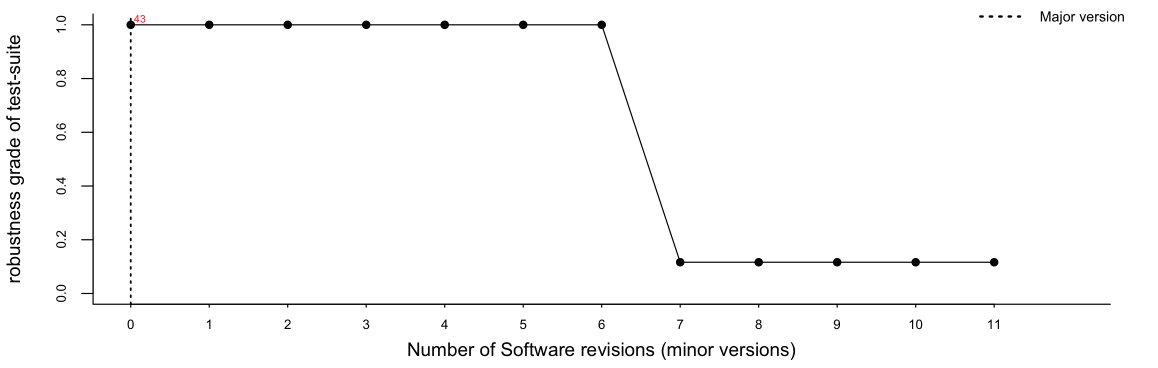
\includegraphics[width=13cm,height=3.05cm]{./Figures/moodle-rq1}}
\vspace{-2mm}\subfigure[Mozilla Marketplace]{\label{rob:fireplace}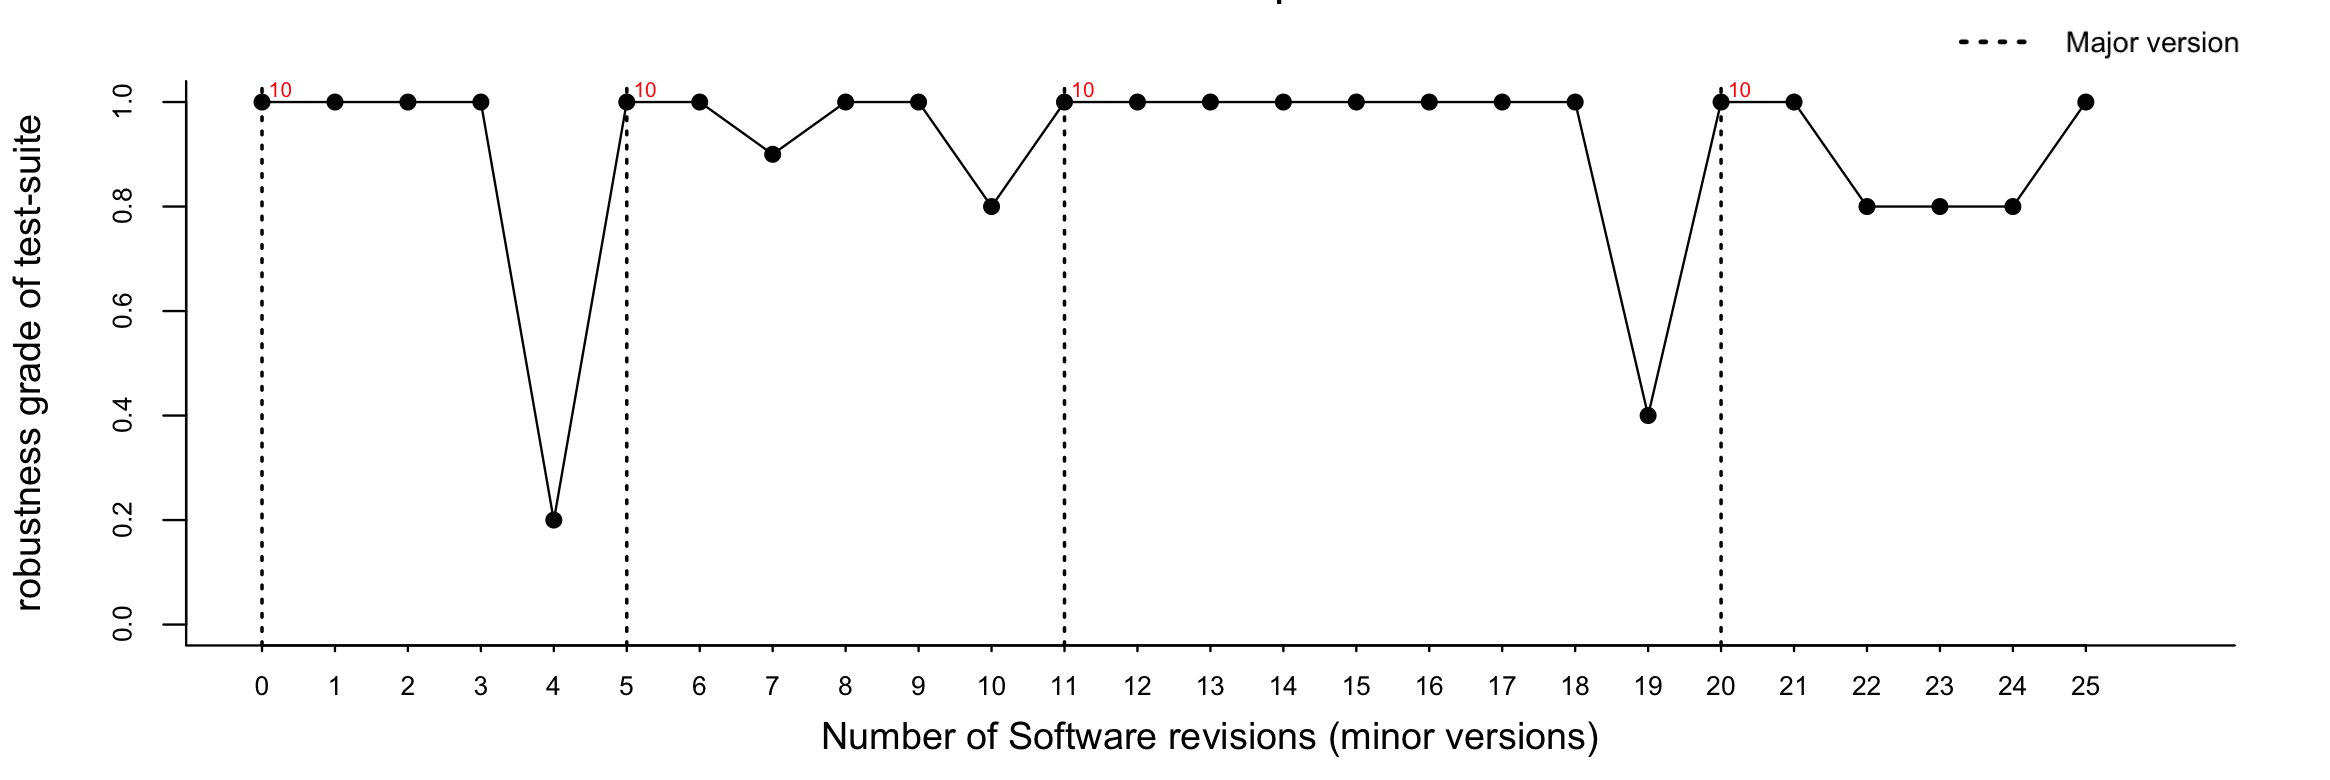
\includegraphics[width=13cm,height=3.05cm]{./Figures/fireplace-rq1}}
\subfigure[Mozilla Addons]{\label{rob:amo}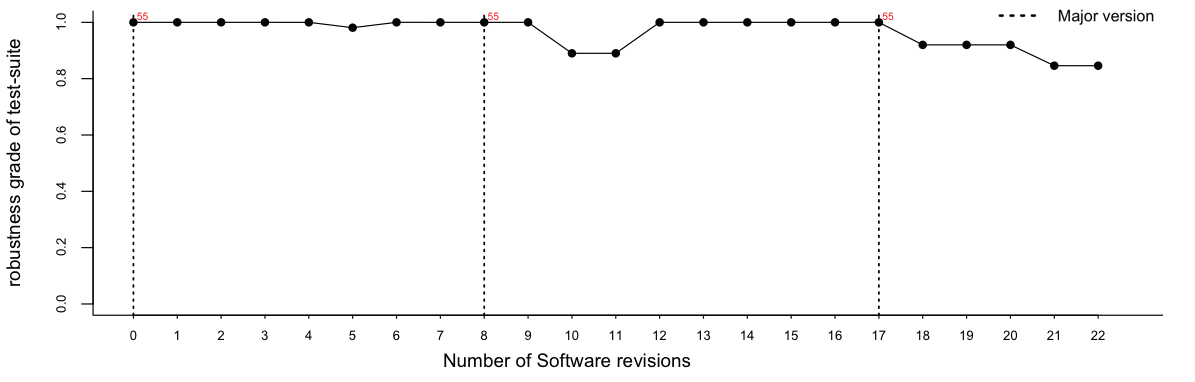
\includegraphics[width=13cm,height=3.05cm]{./Figures/amo-rq1}}
\vspace{-2mm}\subfigure[Mozilla.org]{\label{rob:bedrock}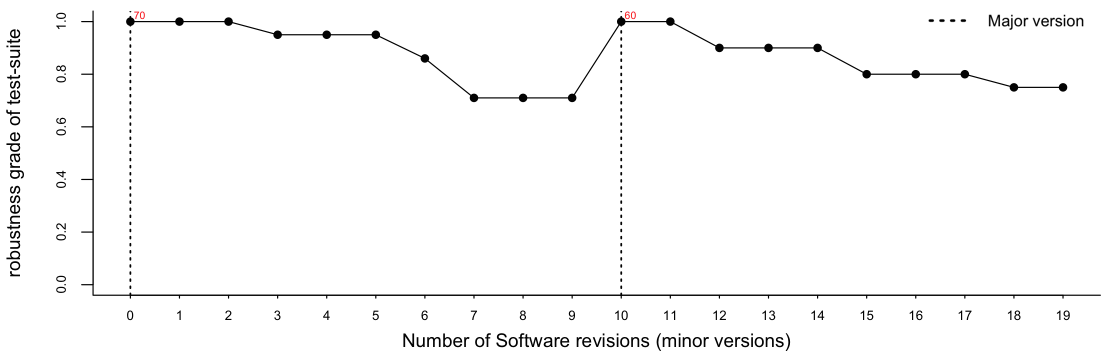
\includegraphics[width=13cm,height=3.05cm]{./Figures/bedrock-rq1}}
\captionsetup{justification=justified,
singlelinecheck=false}
\vspace{-2mm}\subfigure[Jenkins LTS Release Line]{\label{rob:LTS}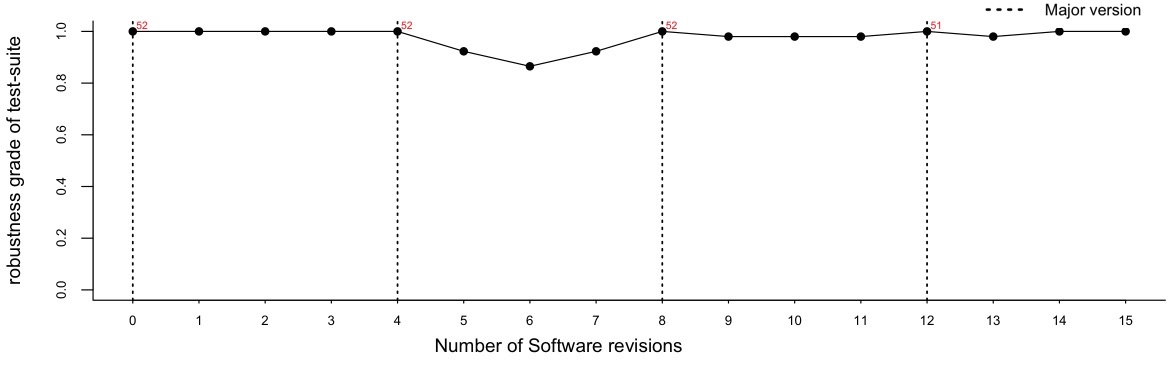
\includegraphics[width=13cm,height=3.05cm]{./Figures/jenkinsLTS-rq1.png}}
\vspace{-2mm}\subfigure[Jenkins Weekly Release Line]{\label{rob:weekly}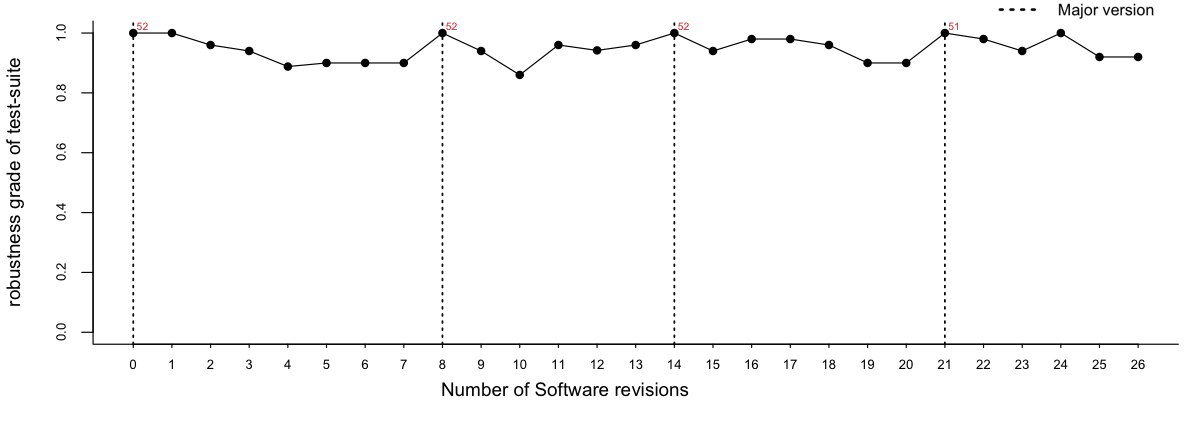
\includegraphics[width=13cm,height=3.05cm]{./Figures/jenkinsWeekly-rq1.png}}
  \captionsetup{justification=justified,
singlelinecheck=false}
\caption{Robustness trend across different revisions of candidate web applications. The x-axis represents software revisions (approximately one year of development history). The dashed vertical line represents major versions. The y-axis represents the robustness grade of the test-suite.}
\label{fig:robustnessplots}
\end{figure} 

A closer look at Figure \ref{rob:moodle} shows that out of all the applications, the robustness grade for Moodle declines the most -- almost 90\% tests were broken from seventh software revision onward. Upon investigation, it was observed that all of these tests used \texttt{xpath} expressions to locate the \texttt{HTML} title attributes of the \textit{anchor} elements. 
Figure \ref{fig:moodleDOM} depicts this change in the structural markup of Moodle between the sixth and seventh software revision, along with the example of missing title attribute (\texttt{title="Add a new user"}). From the seventh revision onward, the \texttt{title} attributes were unavailable and as a consequence, all the tests using \texttt{xpath} locators with \texttt{title} attributes were unable to locate these GUI elements. 
% Remembering from Section \ref{challengesSelenium}, that changes the structural markup of a web-page can affect the robustness of tests. 
% Unfortunately such changes can happen during the evolution of the AUT. 
It was also noticed that the remaining 10\% robust tests in Moodle test-suite implemented only the \texttt{id} element locators. This appears to be the reason why these tests were not broken due to changes in the \texttt{HTML} attributes of the page.
% Upon investigation, it was observed that  due to unavailable \texttt{xpath} expressions (\texttt{NoSuchElementException - xpath}). 
% Remembering from Section \ref{challengesSelenium}, that changing the structural markup of a web-page can affect the robustness of tests. 

% Another 

% \begin{table} 
% \centering
% \begin{tabular}{@{} cl*{12}c @{}}
% %         & & \multicolumn{10}{c}{Test-suite composition} \\[2ex]
% % \hline
%         & & \rot{\textit{id}} & \rot{\textit{xpath}} & \rot{\textit{cssSelector}} & \rot{\textit{name}} & \rot{\textit{tagName}} & \rot{\textit{className}} & \rot{\textit{linkText}} & \rot{\textit{partialLinkText}} & \rot{\textit{sendKeys}} & \rot{\textit{waits}} & \rot{\textit{gets}} & \rot{\textit{clicks}}  \\
% %         \cmidrule{2-12}
% \hline
% 		& Moodle             &w&   &   &   &   &   &  &   &   &  & &w \\
%         & Marketplace               &  &  &  &  &  &  &  &  &  &  & & \\
%         & Addons              &  &   &   &   &  &  &  &   &  &  & & \\
%         & Mozilla.org  &  &  &  &  &  &   &  &  &  &  & & \\
%  \rot{\rlap{~Application}}
%         & Jenkins                & w &   &   &   &   &   &  &   &  &  & &w \\
%         \hline
% %         \cmidrule[1pt]{2-12}
% \end{tabular}
% \caption{Some caption}
% \label{testsuitedistri}
% \end{table}

\begin{figure}[ht!] 
\centering     %%% not \center
\subfigure[Moodle Revision No. 6]{\label{rob:moodleDOm1}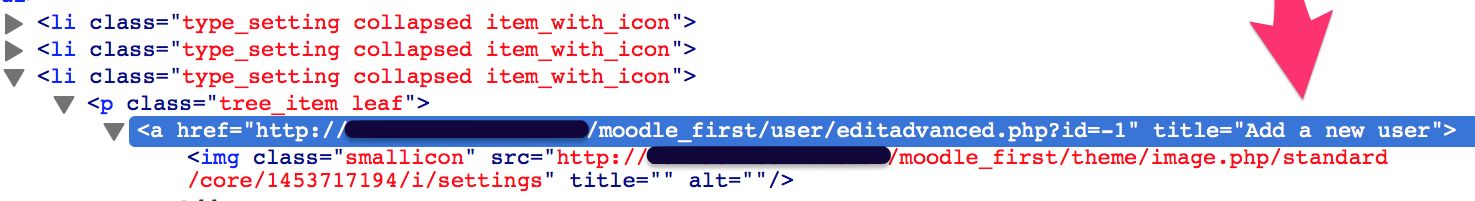
\includegraphics[width=\linewidth]{./Figures/moodle1}}
\subfigure[Moodle Revision No. 7]{\label{rob:moodleDOm2}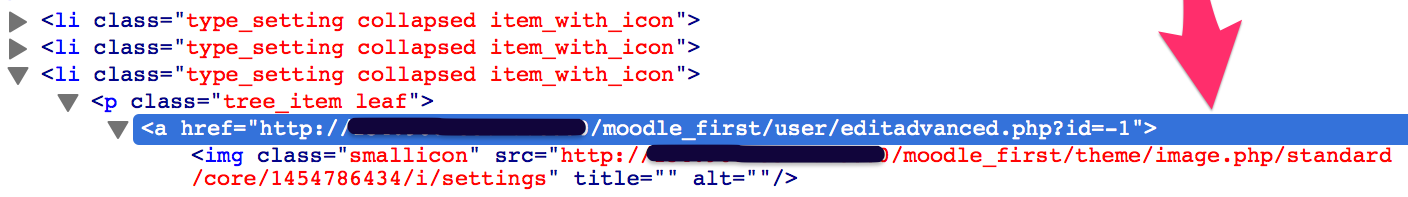
\includegraphics[width=\linewidth]{./Figures/moodle2}}
  \captionsetup{justification=justified,
singlelinecheck=false}
\caption{DOM level differences between two successive software revisions of Moodle. The red arrow highlights the missing \texttt{title="Add a new user"} in Figure (b). (Note: The URL has been stricken through for security reasons.)}
\label{fig:moodleDOM}
\end{figure} 


Changing the manner in which a functionality is accessed also had an effect on the robustness grade of the test-suite. As shown in \ref{fig:bedrockchanges}, between two revisions of Mozilla.org (revision six and seven), a particular `Products' page was no longer accessible through the same URL. This can happen when a certain functionality is moved to another part of the application. Clearly, due to such change, the tests are not able to cover the same functionality. 

\begin{figure}[ht!] 
\centering     %%% not \center
{\label{rob:bedrock1}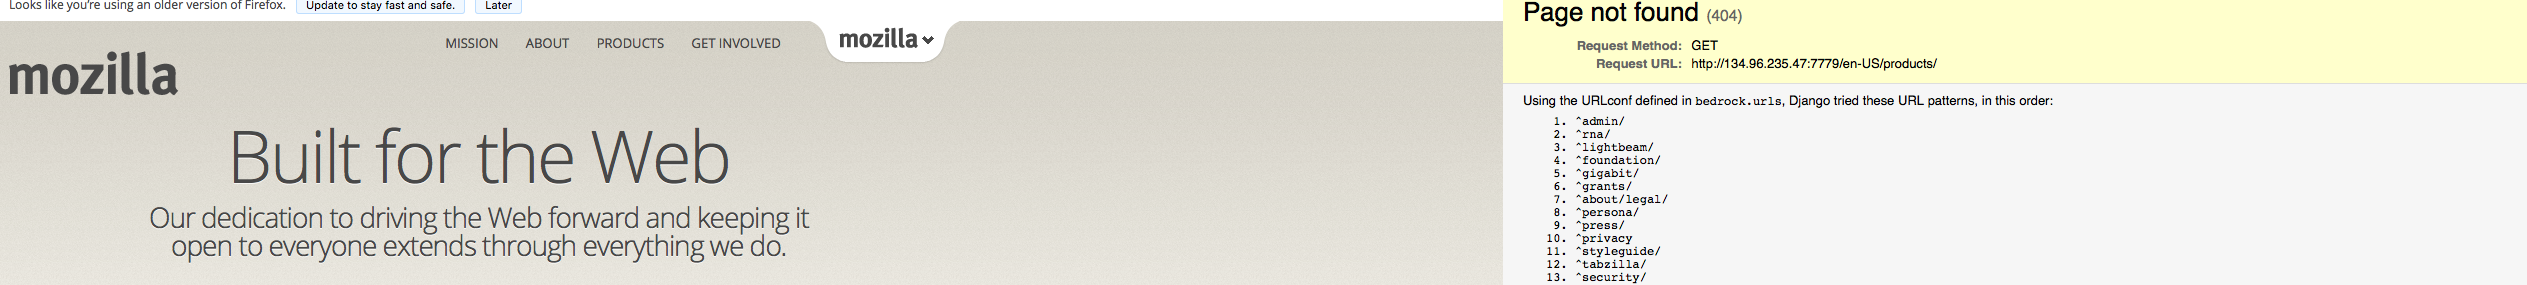
\includegraphics[width=\linewidth]{./Figures/bedrock1}}
\captionsetup{justification=justified,
singlelinecheck=false}
\caption{ The left part of the image shows the `Products' page for Revision No. 6 while the right part shows the `Products' page for Mozilla.org was no longer accessible through the same URL for Revision No. 7.}
\label{fig:bedrockchanges}
\end{figure} 

These examples can be an indication of how GUI level changes in the AUT affect the robustness of tests. Still, one can also observe that for some applications, the robustness trend shows a `dip' in between two minor versions. In other words, the robustness trend appears to go down and go up again. For example, in case of Mozilla Addons, the robustness grade drops between revisions 9 and 11 where some tests are not robust, but the robustness again increases for revision 12. This drop in robustness occurred because a test `timed out' when it was unable to locate a GUI element. Upon investigation, it was observed that the element was indeed present in the DOM, but the test was unable to operate it, which can happen when the element is loaded in the DOM but is not `ready' to interact with. As already mentioned, assessment of such sporadic timing issues is not within the scope of this thesis, since these issues are difficult to reproduce. Nevertheless, it was observed that certain tests are robust if they are run in multiple tries. 


Another factor, page-object pattern, might have contributed towards the overall robustness of the test-suites. All of the candidate test-suites have used this pattern for designing their test-suites. As seen in Table \ref{testsuitedistri}, each test-suite had a very distinct construction but the robustness grades for all the projects show a similar trend. Jenkins tests, for example, included an extensive use of text-inputs, multiple \texttt{click}s and \texttt{get} requests along with actions such as file-uploads, etc. with large action chains (sequential operations on the GUI). Whereas in case of Mozilla.org, since the application is more of an information hub, the ways to interact with the application are limited. Therefore, the tests for Mozilla.org did not use much text inputs and had comparatively short action sequences. Moodle, being a course management system, implemented heavy use of form-validation as well as \texttt{wait} commands in its tests. 

From Table \ref{testsuitedistri} it can be observed that for all the applications the use of \texttt{xpath, css selector} and \texttt{id} locators outnumbers the other locator types. Jenkins and Moodle test-suites use high number of \texttt{xpath} locators, while the three Mozilla test-suites primarily use \texttt{id} and \texttt{css selectors}. Although \texttt{xpath} expressions have not turned out to be as robust in case of Moodle, Jenkins test-suites implement `conditional' \texttt{xpath} expressions (as shown in Listing \ref{jenkinsxpath}) which provide the possibility of locating the same element using different methods. 

\begin{center}
\begin{scriptsize}
\centering
\lstset{
  basicstyle=\ttfamily,
  columns=fullflexible,
  keepspaces=true,
%   frame=none,
}
% \verb|basicstyle=\ttfamily, columns=fullflexible, keepspaces=true|
  
\begin{lstlisting}[caption=Jenkins conditional \texttt{xpath} expression,label=jenkinsxpath]
findElements {using="xpath", value=" .//input[@type='radio'][./@id ='Delegate to servlet container' 
or ./@name = 'Delegate to servlet container' 
or ./@value = 'Delegate to servlet container' 
or ./@placeholder = 'Delegate to servlet container']
}
\end{lstlisting}
\end{scriptsize} 
\end{center}

% As mentioned in Section \ref{stateModelExtraction}, the behavioral state model can only capture \texttt{wait} commands which have a measurable duration. Jenkins test-suite implements two kinds of \texttt{wait} commands -- implicit waits and page-load timeouts\footnote{\url{https://w3c.github.io/webdriver/webdriver-spec.html\#dfn-session-page-load-timeout}}. All other applications use implicit waits in their test-suites. In case of number of \texttt{sendKeys} inputs, the Addons, Marketplace and Mozilla.org test-suites use relatively fewer text inputs. 

The development process of the candidate applications also appears to have an effect on the robustness trend. This can be observed the best with the example of Jenkins LTS and weekly release cycles. In comparison to Jenkins Weekly releases, the tests executed on Jenkins LTS turned out to be more robust. Notice that both release cycles were measured against the same reference major version. As mentioned earlier, the LTS releases had less frequent changes and a more stable development cycle as compared to Jenkins Weekly releases. Such a development process can indicate that the Selenium tests are less prone to break due to the stable structure of the application. 

To sum up, from our observation, approximately half of the first minor versions in the development cycle had a higher robustness grade. Based on that it can be concluded that time itself did not have a greater impact on the robustness as much as the number of incremental changes in the application that resulted in a form of its new minor version. Robustness of the tests was also influenced by factors such as GUI level changes in the AUT and the choice of GUI element locators by certain applications.\\

% Unique GUI locators such as \texttt{id}s may not be available depending upon the structure of the application. 
% From the observation of Moodle, we also realize the importance of . \newline \\
% Another interesting observation about the development cycle of the applications was in case of Mozilla Marketplace. Between the fourth and the fifth revision, the GUI of the application underwent some design changes, as depicted in Figure \ref{fig:fireplacechanges}. During the process, some of the GUI objects such as the placeholder for `Search' field appear to have changed. The test covering the `search' functionality checked the correct placeholder name before performing the search operation. However, due to the aforementioned change, the test failed to assert the presence of the search field, and as a consequence, the test was unable to perform the search function. This observation can be an indication that when an application changes its GUI structure in a manner that alters the GUI objects, the Selenium tests are unable to explore the intended functionality.


% \begin{figure}[ht!] 
% \centering     %%% not \center
% \subfigure[Marketplace Revision No. 4]{\label{rob:fire1}
\includegraphics[width=\linewidth]{./Figures/fireplace1}}
% \subfigure[Marketplace Revision No. 5]{\label{rob:fire2}
\includegraphics[width=\linewidth]{./Figures/fireplace2}}
%   \captionsetup{justification=justified,
% singlelinecheck=false}
% \caption{Changes in the GUI design between two successive software revisions of Mozilla Marketplace. The placeholder for `Search function' changed, and as a consequence the test was unable to perform the search function.}
% \label{fig:fireplacechanges}
% \end{figure} 
% \parskip

\noindent\textbf{RQ1.} How robust are selenium tests against changes of the application under test?
% \subsection{RQ2. Is robustness correlated to the design and composition of the tests?}

The experimental results have shown that the robustness of Selenium tests decreases as an application evolves farther in the development cycle. However, the tests \textit{are} robust enough to stay functional during the first few new releases. Consequently that means that the test will have to be repaired at some later point but there are ways of prolonging the potential robustness level by following practices such as using page-objects, using conditional multi-locators  when unique locators are unavailable, implementing proper setup and tear-down methods in the tests, etc. 

% On a concrete level, the research has shown that approximately half of the first versions in the development cycle had higher robustness grade. Based on that it can be concluded that time itself did not have a greater impact on the robustness as much as the number of improvements on the application that resulted in a form of its new minor version.

% Selenium tests are, therefore, not completely robust against the changes of the AUT but they \textit{are} robust enough to stay unchanged and functional during the first few new releases. Consequently that means that the test will have to be repaired at some later point but the there are ways of prolonging the potential robustness level through other various feature in the structure of the test - which will be explained in the following section. 

% \begin{sidewaysfigure}[ht!] 
% % \centering     %%% not \center
% \subfigure[Moodle Revision 6]{\label{rob:amo}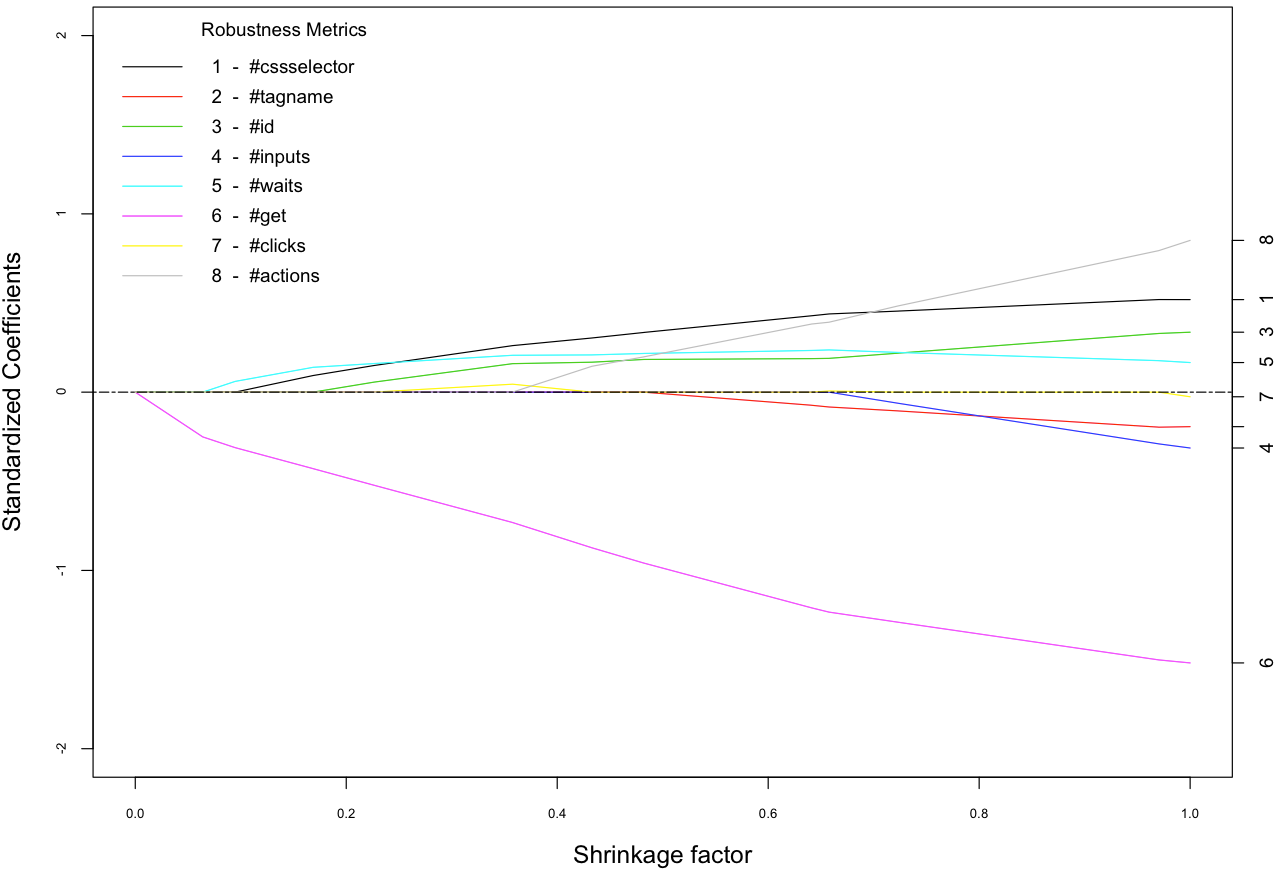
\includegraphics[width=7cm,height=6.2cm]{./Figures/fireplacelasso}}
% \subfigure[Moodle Revision 7]{\label{rob:fireplace}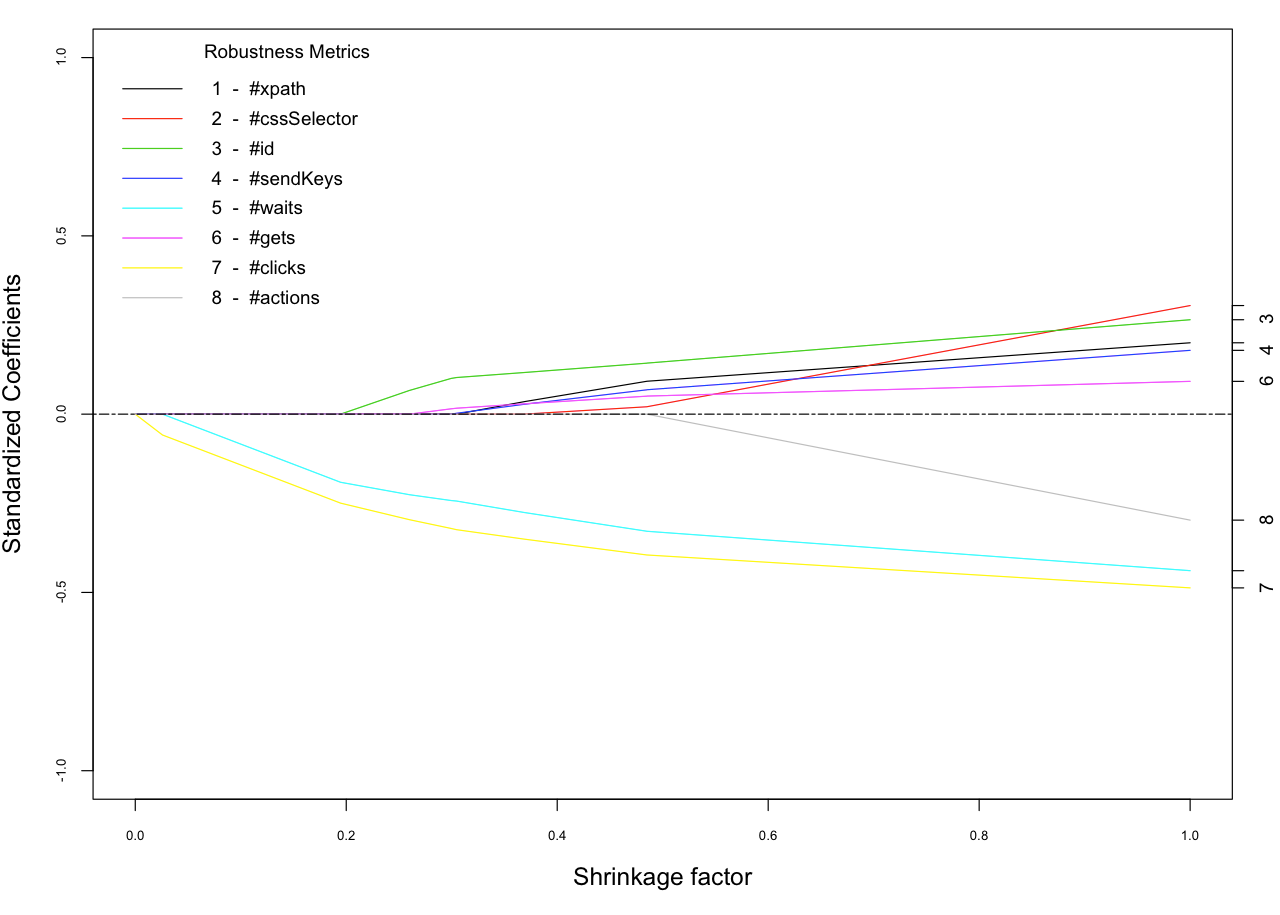
\includegraphics[width=7cm,height=6.2cm]{./Figures/amolasso}}
% \subfigure[Moodle Revision 6]{\label{rob:amo}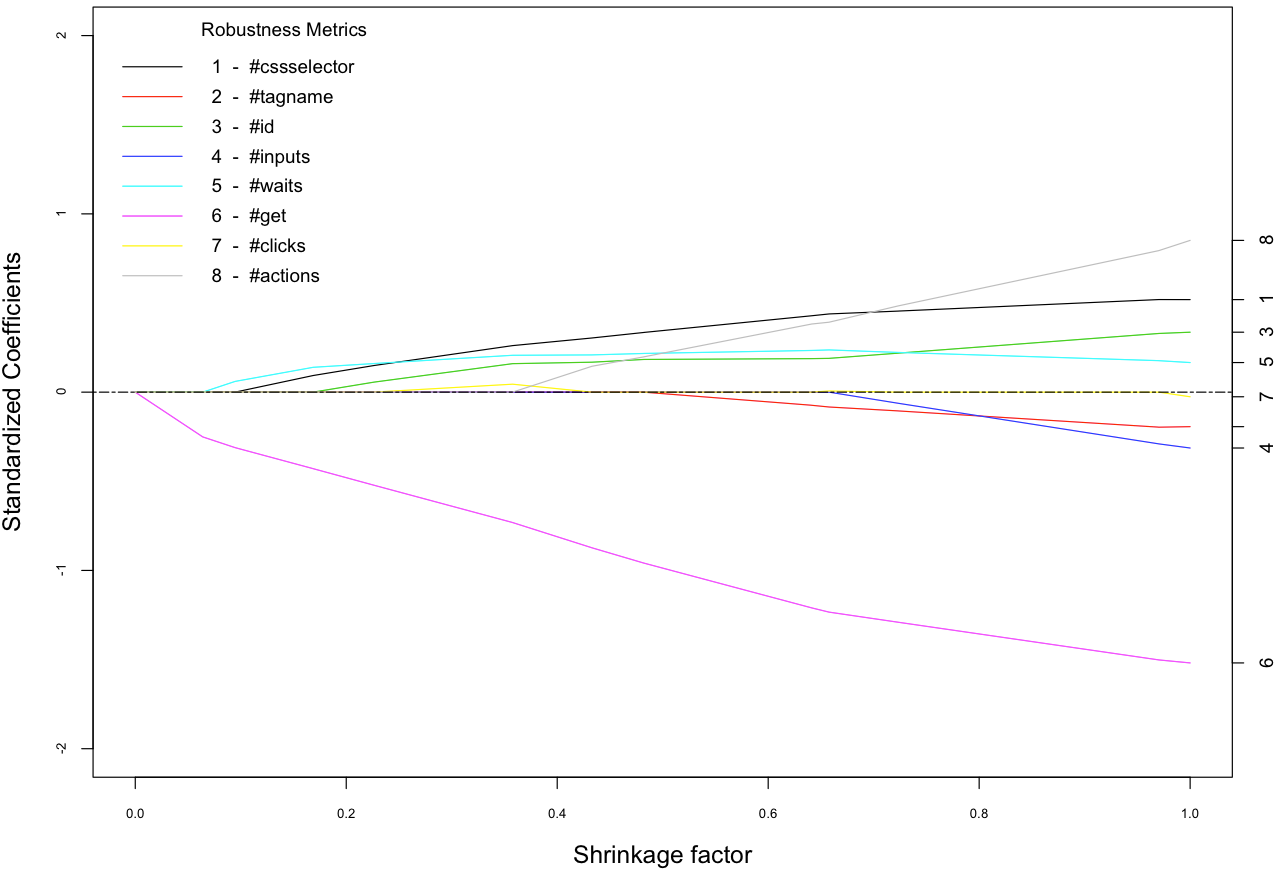
\includegraphics[width=7cm,height=6.2cm]{./Figures/fireplacelasso}}
% \subfigure[Moodle Revision 7]{\label{rob:fireplace}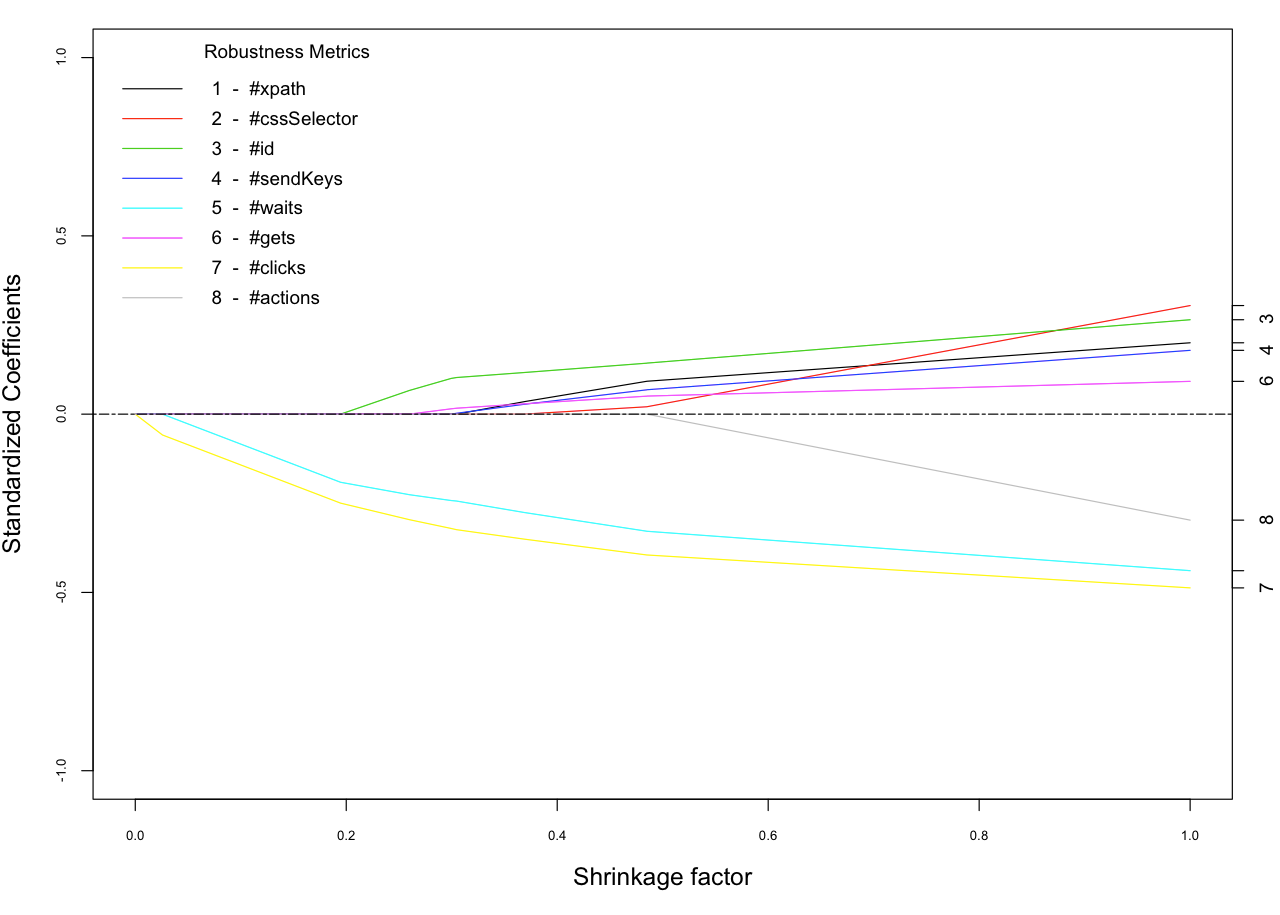
\includegraphics[width=7cm,height=6.2cm]{./Figures/amolasso}}
% \subfigure[Moodle Revision 7]{\label{rob:fireplace}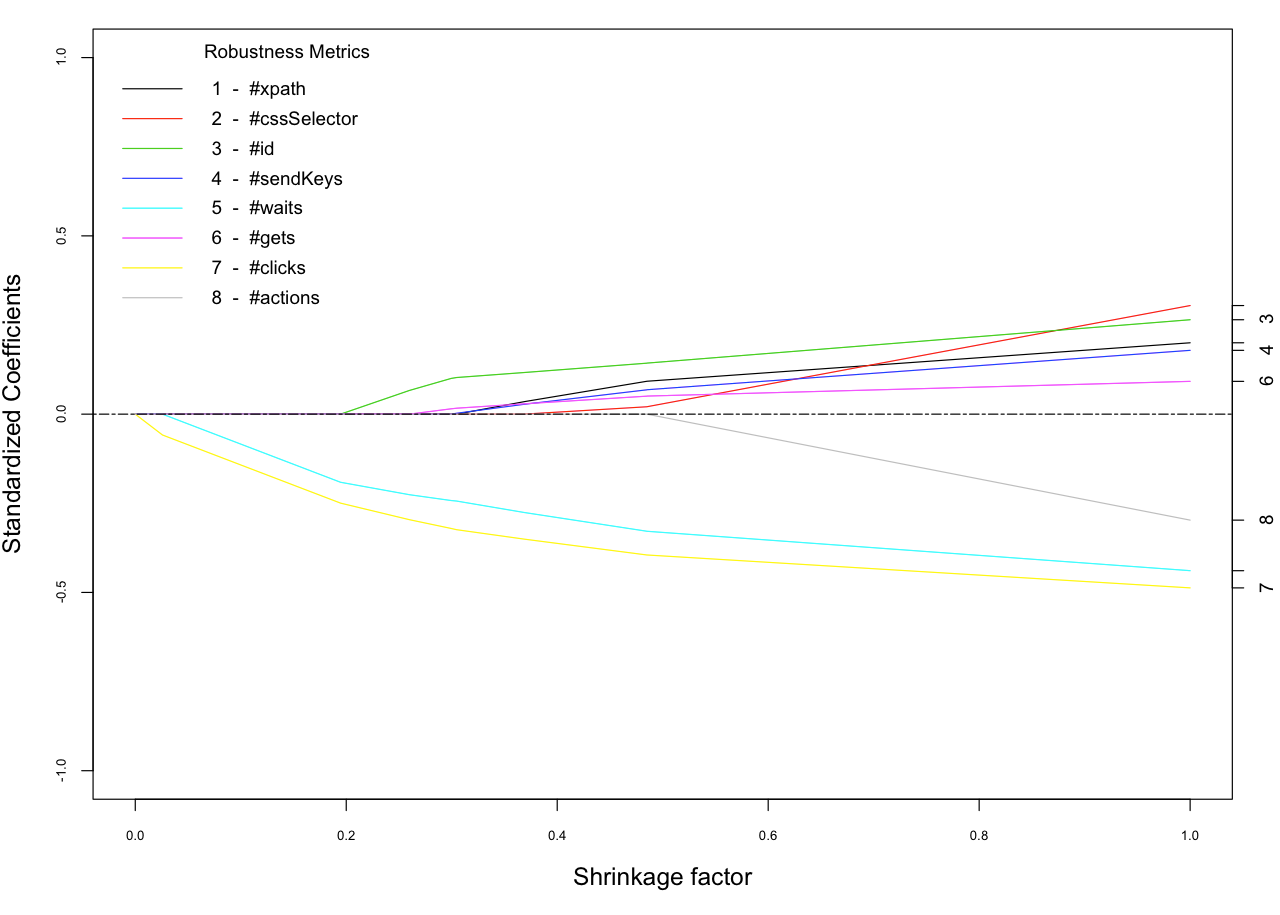
\includegraphics[width=7cm,height=6.2cm]{./Figures/amolasso}}
%   \captionsetup{justification=justified,
% singlelinecheck=false}
% \caption{DOM level differences between two successive software revisions of Moodle. The red arrow highlights the missing \texttt{title="Add a new user"} in Figure (b). }
% \label{fig:moodleDOM}
% \end{sidewaysfigure} 
% \newpage
\subsubsection*{RQ2. Is robustness correlated to the design and composition of the tests?}
%  

To estimate whether there is a correlation between the robustness metrics presented in in Chapter \ref{Chapter3} (Table \ref{rq2metrics}) and the robustness grade of Selenium tests, the implementation approach described in Section \ref{toolimplementation} has been followed. The robustness metrics have been extracted from the behavioral state models and the ground truth (robustness grade of a test) has been established using \texttt{webmate}. The robustness metrics are represented as a feature matrix extended with the ground truth as the solution vector, as depicted in Figure \ref{fig:featurematrix}. The metrics are the independent variables and the robustness grade is the dependent variable using which the statistical analysis has been performed.

The box plot in Figure \ref{fig:spearman} represents the Spearman rank correlation between the robustness of Selenium tests and the proposed robustness metrics which have been developed in Chapter \ref{Chapter3}. Remember that the robustness metrics represent the building blocks of a test's design and composition. The x-axis represents the robustness metrics, while the y-axis reflects the Spearman's rank correlation coefficient for candidate web applications. As mentioned in Section \ref{sec:Statistical}, a high correlation coefficient indicates that when value of one variable increases, value of other variable increases as well. While a high negative value indicates that when value of one variable increases, value of other variable decreases. A value close to zero indicates that the two variables are statistically independent. 
% It should be noted that correlation does not imply causation. 

Each box also represents the `spread' of the Spearman's correlation coefficient for each metric across the candidate applications (data sets). The horizontal lines inside the boxes represent `median' correlation coefficient. The vertical bars (`whiskers') stretching out on both sides of the box represent the `range' of the values of the correlation coefficient. The stand-alone point indicates `outlier', i.e. value which lies outside the `range' -- farther than one and half times the length of the box. 

A closer look at the box plot reveals the median correlation coefficient for most of the metrics lies between [-0.2, 0.2]. The metrics \textit{\#name} and \textit{\#tagName} only have one and two coefficient values, respectively. This is due to the fact that the GUI element locator \texttt{name} is used only in Jenkins test-suite, while \texttt{tag name} locator is used only by Mozilla Marketplace and Jenkins (this can be observed in Table \ref{testsuitedistri}). Similarly, not all metrics are applicable on all applications. Metrics where the standard deviation is zero, are not included during the correlation computation. This is because a standard deviation of zero indicates that the metric has no spread (e.g. all sample values are the same) and that it would not have any influence on the dependent variable. This is the case for metrics \textit{\#partialLinkText}, \textit{\#linkText} and \textit{\#className}. As it can be observed, out of all the metrics, \textit{\#name} and \textit{\#tagName} correlation coefficients are very close to zero. This indicates that these metrics may have a very weak influence on the robustness grade. 

\begin{figure}[ht!] 
\centering     %%% not \center
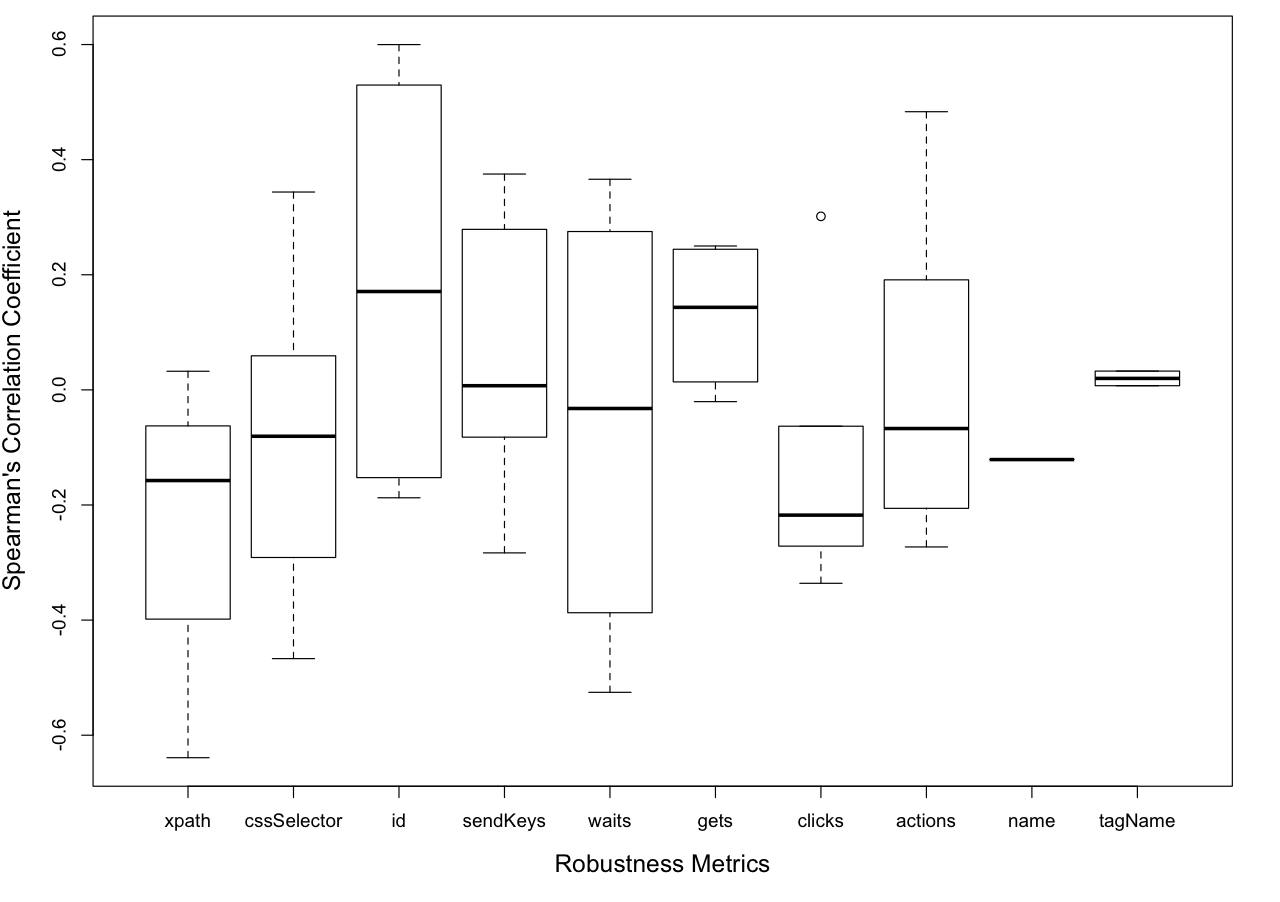
\includegraphics[width=15cm,height=10cm]{./Figures/spearman-rq2}
 \captionsetup{justification=justified,
singlelinecheck=false}
\caption{Spearman correlation box plot. The x-axis represents the robustness metrics and the y-axis represents the Spearman's correlation coefficient. (Note: For better readability, the `\#' sign has been omitted from the metrics' names.)}
\label{fig:spearman}
\end{figure} 

% \subsection{Design and Composition of tests}

In statistics, the function \textit{p-value} can be used to determine the significance of the outcome of a test. In case of correlation, a small p-value can indicate an evidence against the null hypothesis.
In the observed correlation coefficients, the metric \textit{\#xpath} has two coefficients of -0.63 (Moodle), -0.15 (Addons) which have p-values $<$ 0.005. Whereas the metric \textit{\#id} has strongest positive correlation of +0.59 with p-value $<$ 0.005. This coefficient represents the Moodle data set. Recalling from previous section, all of the tests using \texttt{id} locators in Moodle test-suite were robust. 


% In case of \textit{\#cssSelector} the two of the moderate correlation coefficients of -0.466 (Mozilla.org) and -0.29 (Moodle) have p-values $<$ 0.05. 

% For the metric \textit{\#waits} the correlation coefficient shows a high standard deviation, the p-values for positive correlation coefficients 0.36 and 0.18 are $>$ 0.2, while the p-values for negative correlation coefficients -0.52 and -0.24 are $<$ 0.001.  
% Remembering that this metric represents the number of \texttt{wait} commands in a test, a negative correlation suggests that higher number number of \texttt{wait} commands in a test might decrease its robustness. 

For metrics with large deviations in the correlation coefficients (e.g. in case of \textit{\#cssSelector, \#sendKeys, \#waits}) it is complicated even more to interpret the influence the metric has on robustness grade. Two important factors affecting this behaviors are the sample size of each test-suite and the overall robustness of the tests. Consider the metric \textit{\#sendKeys} for example. For this metric the correlation coefficient of -0.28 for Addons was observed with p-value $<$ 0.005 while the correlation coefficient of 0.27 for Moodle, the p-value was $>$ 0.6. For both of these applications, the histograms in Figure \ref{fig:AddonsHist} and \ref{fig:moodleHist} depict the difference in the distribution of robustness grade. From previous section we remember that almost 90\% of tests for Moodle were not robust for half of the minor versions while almost 90\% of the Addons tests were robust. In such situations, a p-value may not fully indicate the strength of the rank correlation. For the remaining correlation coefficients, the observed correlation was either weak (coefficient between -0.10 to 0.10) or the p-values were high ($>$ 0.4). 

\begin{figure}[htb!] 
\centering     %%% not \center
\subfigure[Mozilla Addons]{\label{fig:AddonsHist}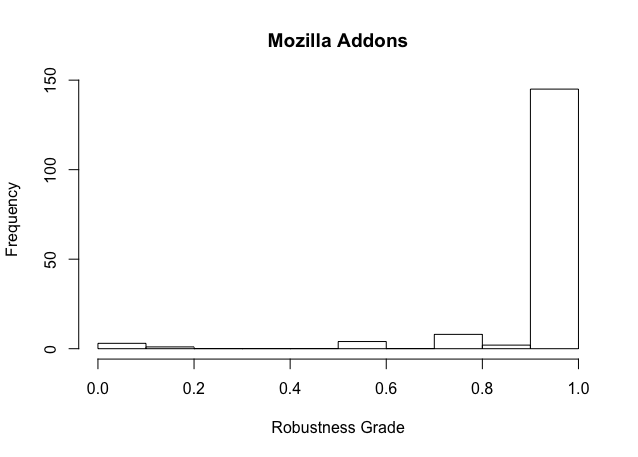
\includegraphics[width=7cm,height=5cm]{./Figures/AddonsHist}}
\subfigure[Moodle]{\label{fig:moodleHist}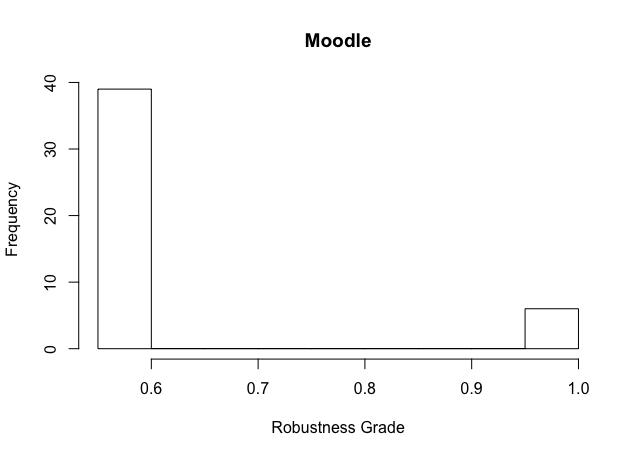
\includegraphics[width=7cm,height=5cm]{./Figures/moodleHist}}
  \captionsetup{justification=justified,
singlelinecheck=false}
\caption{Histogram distributions of robustness grade for Mozilla Addons and Moodle. The x-axis represents robustness grade and y-axis represents the frequency.}
\label{fig:hist}
\end{figure} 

A large deviation from the x-axis further indicates that for a given metric, the correlation coefficient takes negative and positive values for different applications. From the observed data, it is therefore not straightforward to determine the significance of the correlation between the metrics and the robustness grade. From what we have observed in the previous section, with the exception of Moodle, other test-suites were relatively robust. This implies that for majority of the tests from these test-suites, the dependent variable (robustness grade) was equal to one despite the changes in the distribution of the independent variables. In this case, there are many `ties' in the ranks of the ordered variables, which can affect the computation of the correlation coefficient. 

To verify whether the above-mentioned observation is due to the ties in the ranking, we can compute the correlation coefficient which is not affected by the ties, such as Pearson's correlation coefficient. However, it should be noted that Pearson's correlation requires a linear relationship between two variables, which might not hold true for every metric. Figure \ref{fig:pearson} represents the box plot for Pearson's correlation coefficient. As we can see, the spread of the coefficients is shorter as compared to Spearman's coefficients for most of the metrics while the median values are closer to zero as compared to Spearman's coefficients. These differences can occur on account of not meeting the assumptions of Pearson's correlation (e.g. linearity) by certain variables. Overall, the distribution of the correlation coefficients do not appear to indicate any surprising differences between these two correlation methods. As a result, it is nevertheless intricate to draw a direct conclusion about the correlation from these coefficients. 

\begin{figure}[ht!] 
\centering     %%% not \center
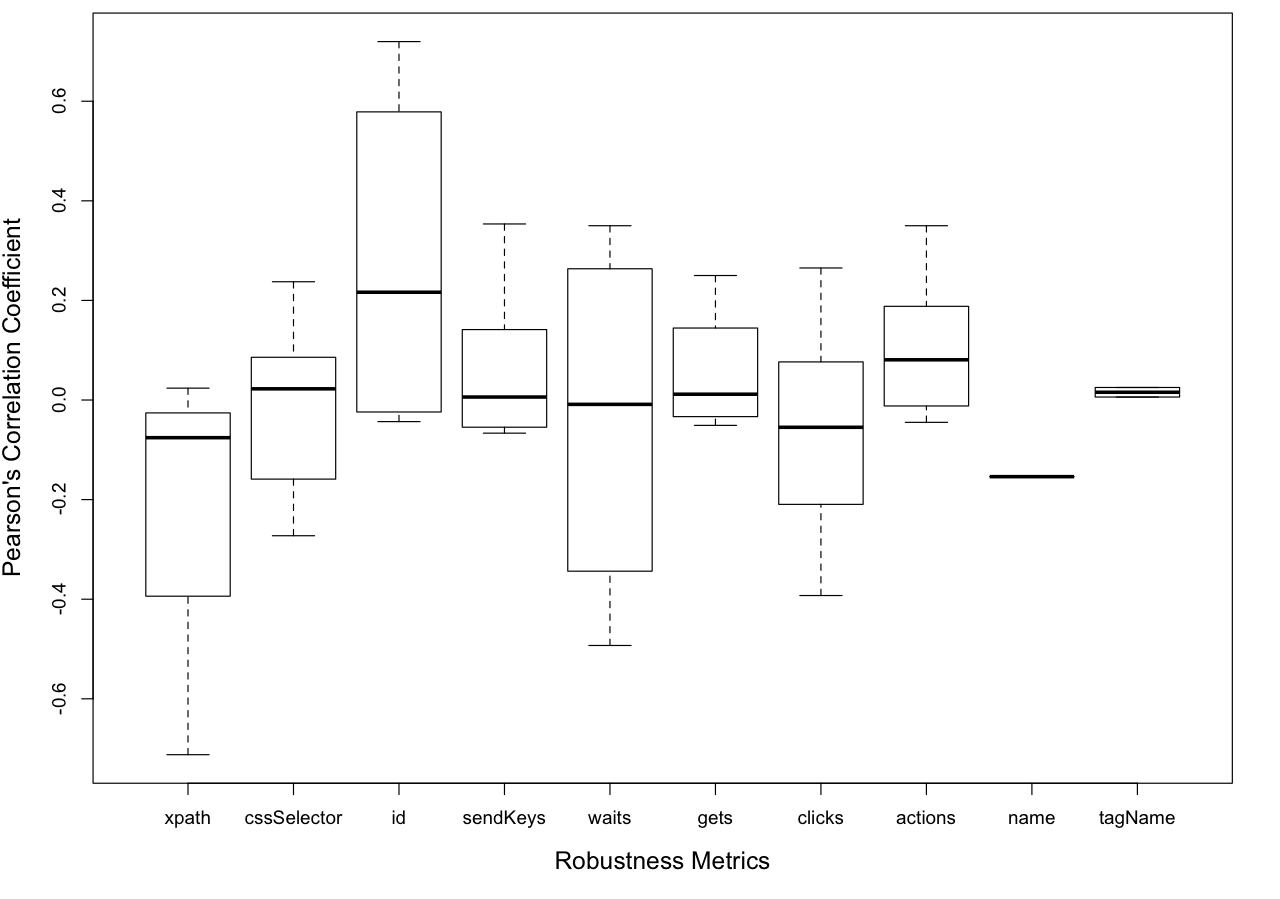
\includegraphics[width=15cm,height=10cm]{./Figures/pearson-rq2}
 \captionsetup{justification=justified,
singlelinecheck=false}
\caption{Pearson correlation box plot. The x-axis represents the robustness metrics and the y-axis represents the Pearson's correlation coefficient. (Note: For better readability, the `\#' sign has been omitted from the metrics' names.)}
\label{fig:pearson}
\end{figure}

It is possible that some of the metrics are strongly correlated with each other whereas some metrics convey more meaningful information about the robustness than other metrics. Therefore a subset of most significant metrics can be identified. As mentioned in Section \ref{regression}, to identify the most influential metrics, the \textit{lasso} shrinkage method has been applied. All the data sets for candidate applications have been standardized, as described in Section \ref{datasetstandardization}. 

Figures \ref{fig:lasso1}, \ref{fig:lasso2}, and \ref{fig:lasso3} represent the \textit{lasso} shrinkage models for candidate web applications. Each `lasso path' on the graphs depicts a robustness metric represented by a distinct color. The legend on the top-left corner represents the robustness metrics. The x-axis represents the shrinkage factor and the y-axis represents standardized correlation coefficients between a metric and the robustness grade. Metrics with higher positive or negative correlation coefficients can have more influence on the shrinkage model whereas metrics with coefficients close to zero are weighted lower in the model. To assess the impact a metric has on the model, we can observe the point at which a metric's `lasso path' aligns with the x-axis. This is the point at which a metric's coefficient \textit{shrinks} to zero. Observing from right-to-left side, the later a metric's `lasso path' aligns with the x-axis, the more impact it has on the shrinkage model. 

As explained earlier, not all metrics are applicable on all projects, some metrics are not used by certain projects or they have standard deviation of zero, and hence are not included in the model. After looking at Figures \ref{fig:lasso1} (Moodle), \ref{fig:lasso2} (Mozilla Marketplace and Addons), and \ref{fig:lasso3} (Jenkins and Mozilla.org), the primary observation is that each candidate application has a different metric with the most impact on the model. In other words, none of the applications shares a common, most influential predictor. This could be the case because for each model, the same predictor can have different `weight' depending upon the influence of other variables in the data set. There are certain metrics which are shared commonly across the projects but do not have the same impact on each model. Consider the metric \textit{\#actions} --  remembering from Section \ref{test-actions}, number of `actions' indicated the number of GUI sequences executed by the test. Our idea behind this metric was that higher number of actions in a test would make it less robust. This idea is supported by Mozilla Addons where the \textit{\#actions} has a negative correlation. However, the remaining projects Jenkins and Mozilla.org show contradictory information as  \textit{\#actions} has a positive correlation. 

A closer look at the metrics across all the applications reveals that although there is no common, single most influential predictor among the projects, some projects do share a common set of influential predictors in their top-five predictors. As an example, in case of Moodle, the metric \textit{\#id} has the highest influence for predicting a test as robust. This metric indicates the number of \texttt{id} locators implemented in a test. The metric is also shared among the top-five metrics for Mozilla Addons and Mozilla Marketplace with positive correlation. Jenkins did not use any \texttt{id} locators as we have seen in previous section. While in case of Mozilla.org, the correlation for \textit{\#id} is close to zero. This indicates that for three out of four projects, the higher number of \texttt{id} locator implementations in a test, the more robust a test was while the metric had virtually no influence on the model for Mozilla.org. 

\begin{figure}[ht!] 
\centering     %%% not \center
{\label{fig:moodlelasso}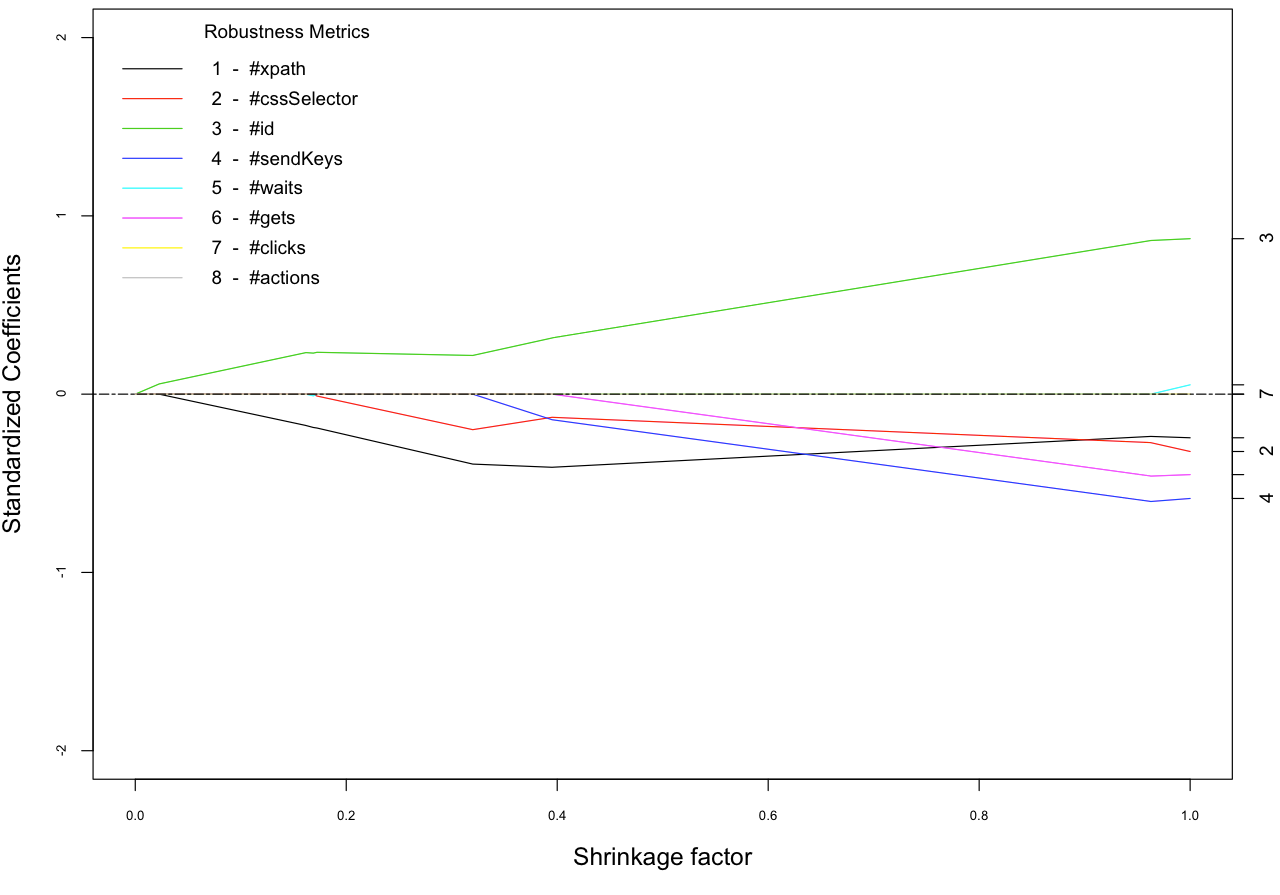
\includegraphics[width=13cm,height=10cm]{./Figures/moodlelasso}}
  \captionsetup{justification=justified,
singlelinecheck=false}
\caption{The \textit{lasso} shrinkage model for Moodle. The x-axis represents the shrinkage estimation and the y-axis represents standardized correlation coefficients. The legend on the top-left corner represents the enumerated robustness metrics, as reflected on the secondary y-axis.}
\label{fig:lasso1}
\end{figure} 


\begin{figure}[tbp!] 
\centering     %%% not \center
\subfigure[Mozilla Marketplace]{\label{fig:fireplacelasso}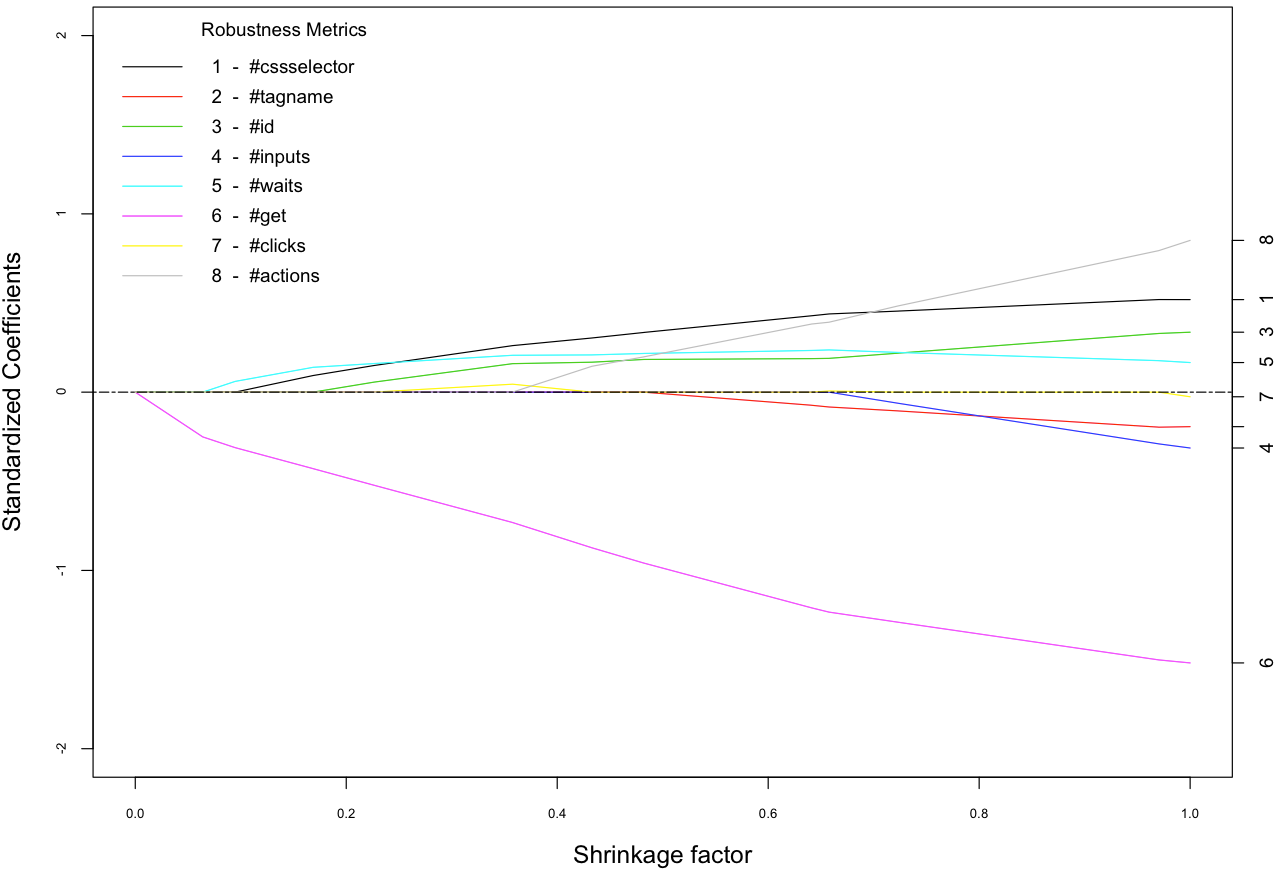
\includegraphics[width=13cm,height=9cm]{./Figures/fireplacelasso}}
\subfigure[Mozilla Addons]{\label{fig:amolasso}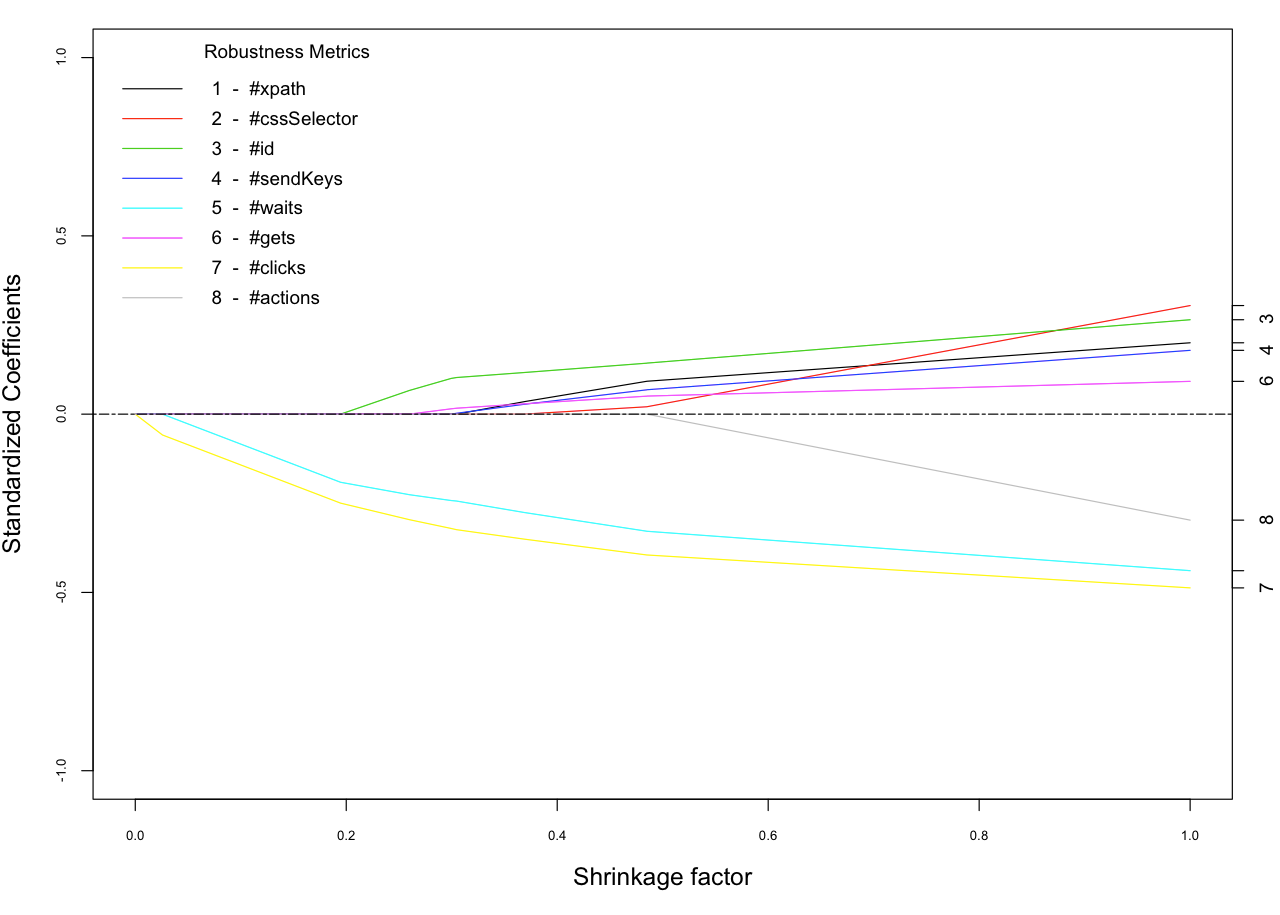
\includegraphics[width=13cm,height=9cm]{./Figures/amolasso}}
  \captionsetup{justification=justified,
singlelinecheck=false}
\caption{The \textit{lasso} shrinkage models for Mozilla Marketplace and Mozilla Addons. The x-axis represents the shrinkage estimation and the y-axis represents standardized correlation coefficients. The legend on the top-left corner represents the enumerated robustness metrics, as reflected on the secondary y-axis. }
\label{fig:lasso2}
\end{figure} 

\begin{figure}[htbp!] 
\centering     %%% not \center
\subfigure[Jenkins]{\label{fig:jenkinslasso}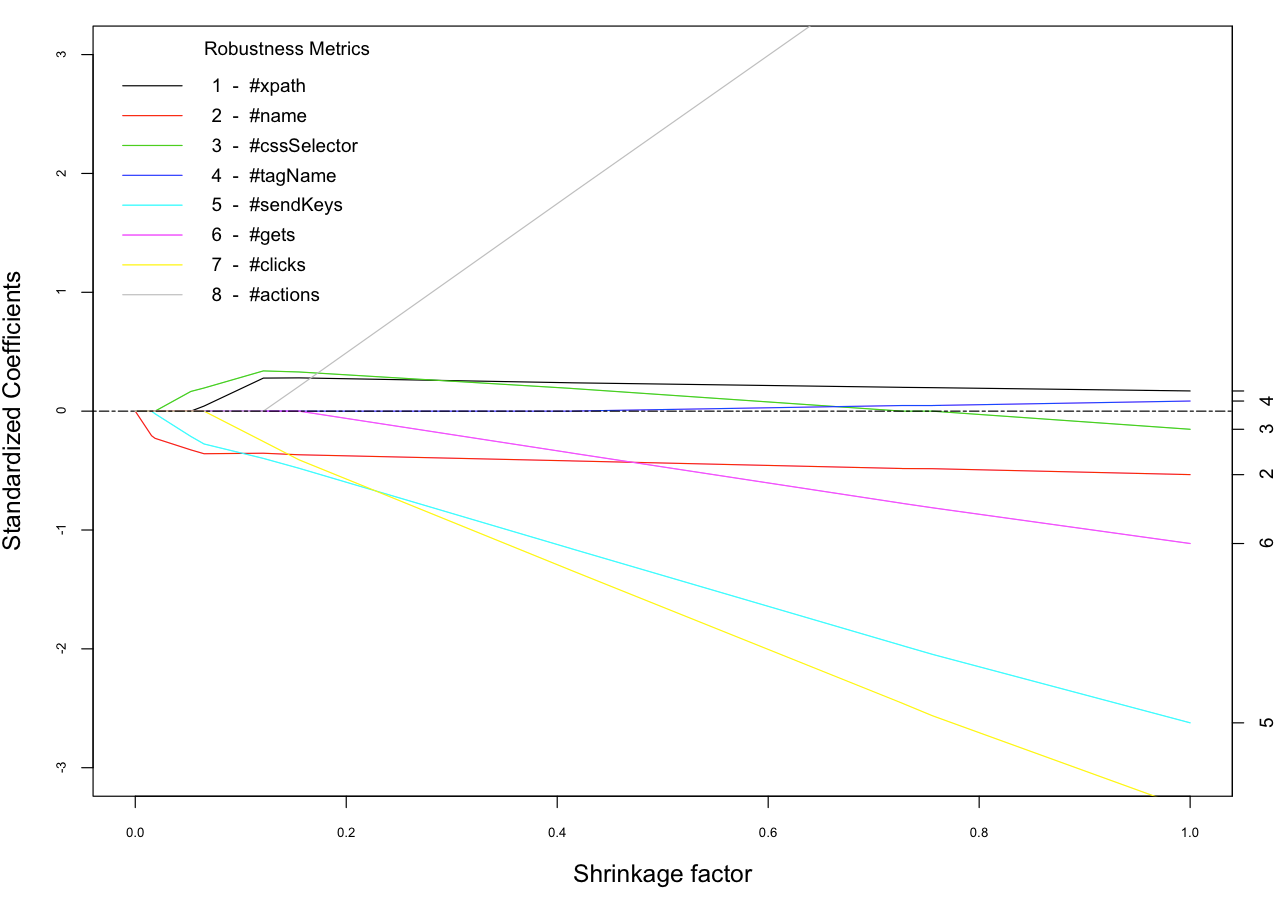
\includegraphics[width=13cm,height=9cm]{./Figures/jenkins}}
\subfigure[Mozilla.org]{\label{fig:bedrocklasso}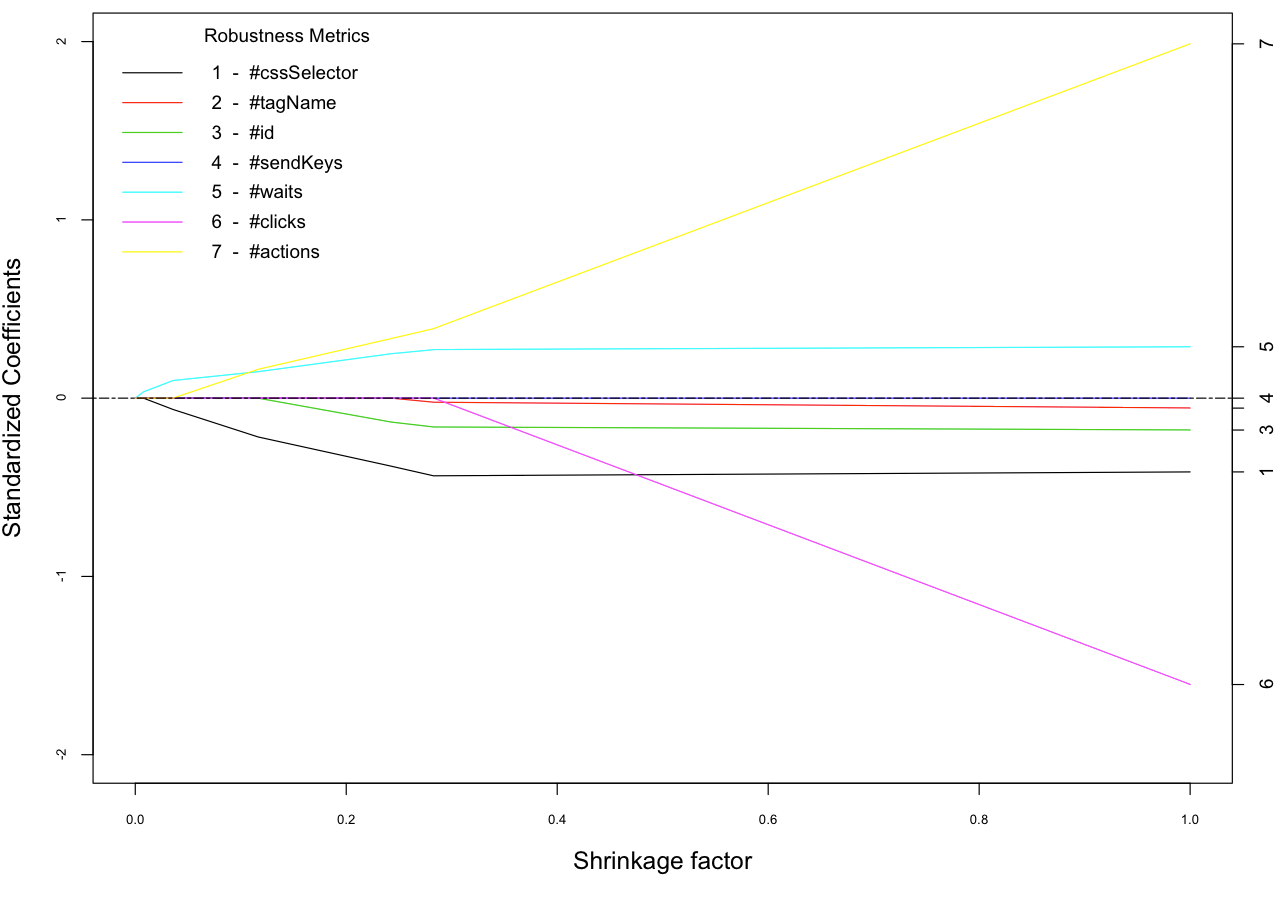
\includegraphics[width=13cm,height=9cm]{./Figures/bedrocklasso}}
  \captionsetup{justification=justified,
singlelinecheck=false}
\caption{The \textit{lasso} shrinkage models for Jenkins and Mozilla.org. The x-axis represents the shrinkage estimation and the y-axis represents standardized correlation coefficients. The legend on the top-left corner represents the enumerated robustness metrics, as reflected on the secondary y-axis. } 
\label{fig:lasso3}
\end{figure} 

Another common metric for the projects is \textit{\#clicks}. The assumption behind introducing this metric was that lower 
number of state-changing actions such as a \texttt{click} can make a test more robust. Thus a negative correlation for \textit{\#clicks} would support this assumption. For the projects Jenkins, Mozilla.org and Mozilla Addons, this metric has negative correlation whereas for Mozilla Marketplace and Moodle, the correlation is close to zero and the coefficients are shrunk to zero very early in the models, implying that these metrics were highly correlated with other metrics. For Mozilla Addons, this metric is the most influential metric. 

In case of the metric \textit{\#cssSelector}, yet again there is contradictory evidence -- for Mozilla Marketplace and Addons there is a weak positive correlation, while for other projects the metric is negatively (weak) correlated. The metric \textit{\#gets} has the highest impact on the model of Mozilla Marketplace. Remember from Section \ref{test-actions}, a \texttt{get} request changes the state of the AUT, such as navigating to a different web page. The assumption behind introducing this metric was that high number of \texttt{get} requests in a test can decrease the robustness of a test. The negative correlation coefficients of this metric for Mozilla Marketplace, Jenkins and Moodle seem to confirm this assumption, while in case of Mozilla Addons, the coefficients are positive but very close to zero. The metric \textit{\#xpath} has very weak positive correlation coefficients for Jenkins and Mozilla Addons and weak negative coefficients for Moodle. From the results of previous section, we can interpret these coefficients, since the Jenkins test-suite used \texttt{xpath} expressions and was relatively robust, while the Moodle tests using \texttt{xpath}s turned out to be not robust. 

Metric \textit{\#sendKeys}, which represents number of text inputs, shows negative correlations for Jenkins and Moodle, while the coefficients for other projects are very close to zero. Thus, from these two observations, we can conclude that the higher number of text inputs in a test, the less robust the test is. 
In case of the remaining metrics \textit{\#name, \#tagName} do not seem so informative since there is very low correlation combined with the fact that these metrics are used by only two projects. \\
%  

% A positive correlation coefficient indicates that more the number of text inputs in a test the more robust the test was. From previous section we remember that almost 90\% of tests for Moodle were not robust for half of the minor versions while only six tests were fully robust as seen in Figure \ref{fig:moodleHist}. Hence the p-values do help to assess the strength of the correlation in this situation.


\noindent\textbf{RQ2.} Is robustness correlated to the design and composition of the tests?

The statistical analysis for the purposes of this thesis has shown that no specific metric in the design and composition of the test correlates directly with the robustness grade. 
Therefore, none of the observed metrics solely is able to predict that the Selenium test will remain robust throughout the testing of the version history of an AUT.

However, we have also observed that compositions of some tests were more robust than the other ones. Additionally, it has been noticed that the same metrics that had a high influence on the robustness for a certain AUT did not have any significant impact on the robustness on another AUT. The shrinkage models were able to identify a set of top metrics among all candidate applications -- in particular the \textit{\#id} and \textit{\#clicks} metrics. Therefore, it can be concluded, after all, that a \textit{combination of metrics} in the composition of certain tests definitely can contribute to higher robustness grade.
% The research for the purposes of this thesis has shown that no specific factor in the design and composition of the test correlates directly with a higher robustness grade of an AUT -- regardless the context. Therefore, none of the observed factors solely is able to guarantee that the Selenium test will remain successful throughout the testing of the history versions of an AUT.

%However, we have also seen that compositions of some tests were more stable than the other ones as well as it has been noticed that the same metrics that had made tests of a certain AUT stable did not have any significant impact on the robustness at all in a group of tests performed on another AUT. 

%Although no independent constant can be derived from the results, it can be concluded, after all, that a combination of metrics in the composition of certain tests which are in accordance with the nature of the AUT definitely can contribute to higher robustness grade. 

% \label{robustnessresults} 





 

\begin{figure}[htbp!] 
\centering     %%% not \center
\vspace{-0.4cm}
\subfigure[Mozilla Marketplace]{\label{rq3:fireplace}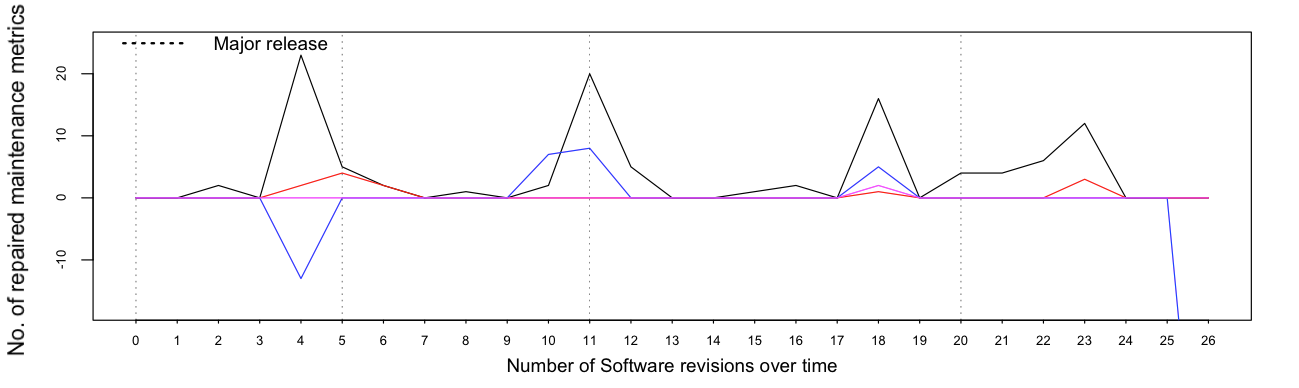
\includegraphics[width=14cm,height=3.9cm]{./Figures/fireplacerq3.png}}
\subfigure[Mozilla Addons]{\label{rq3:amo}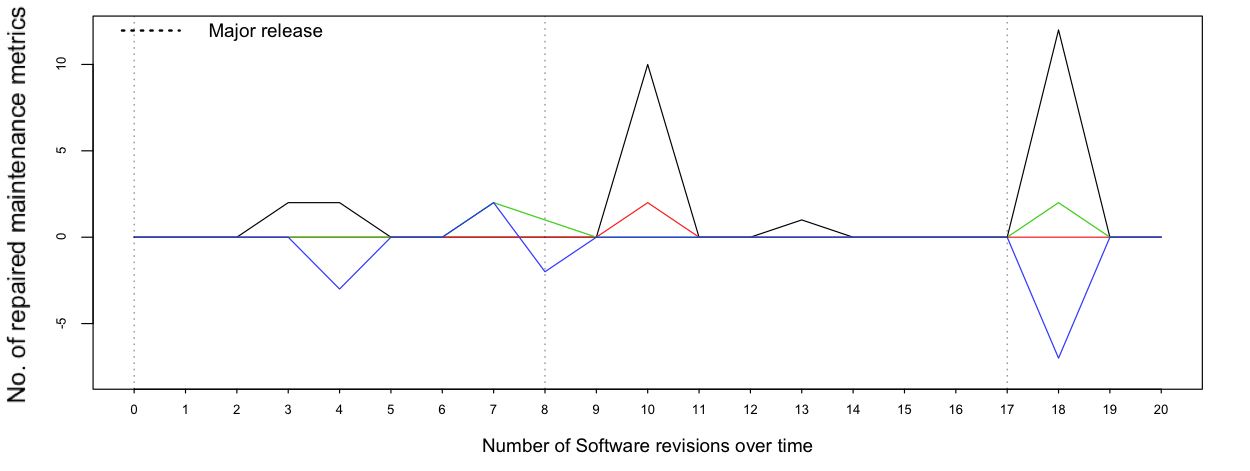
\includegraphics[width=14cm,height=3.9cm]{./Figures/amorq3.png}}
\subfigure[Mozilla.org]{\label{rq3:bedrock}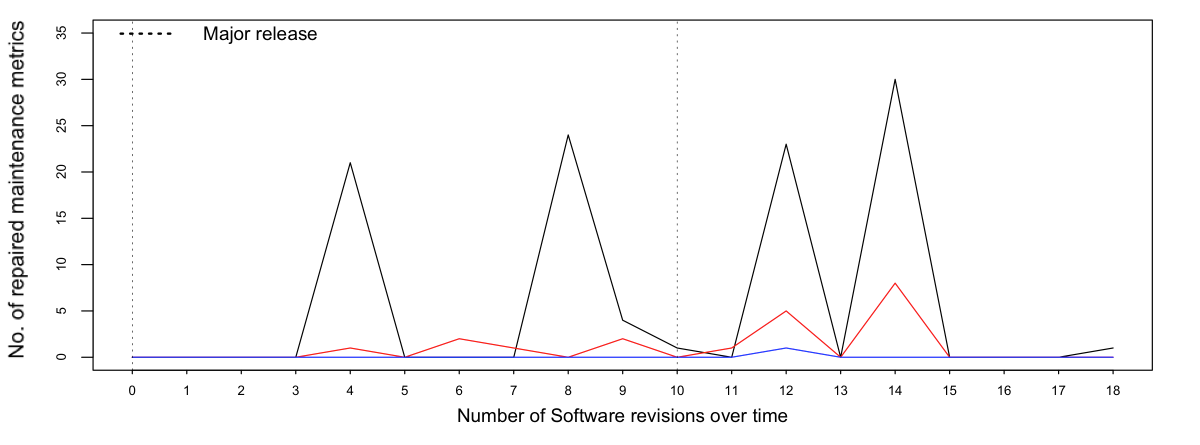
\includegraphics[width=14cm,height=3.9cm]{./Figures/bedrockrq3.png}}

\subfigure[Jenkins]{\label{rq3:weekly}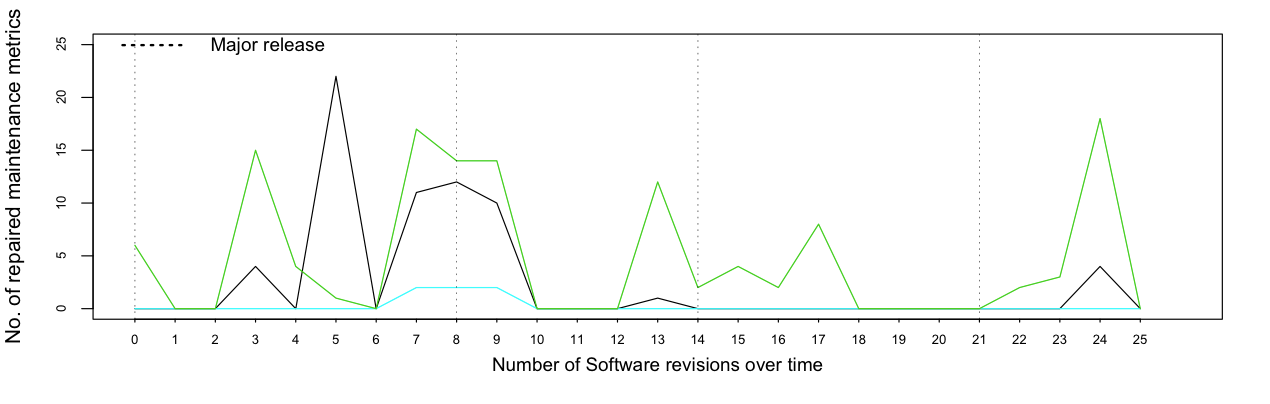
\includegraphics[width=14cm,height=3.9cm]{./Figures/jenkinsrq3.png}}
\subfigure[Legend: Metric names]{\label{rq3:myleg}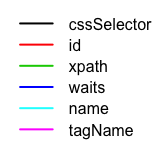
\includegraphics[width=3.5cm,height=1.9cm]{./Figures/myleg.png}}

  \captionsetup{justification=justified,
singlelinecheck=false}
\caption{Maintenance metrics for Selenium test-suites. The x-axis represents software revisions. The dashed vertical line represents major versions. The y-axis represents the number of maintenance metrics repaired. Legend \ref{rq3:myleg} is applicable on all Figures.} 
\label{fig:rq3plot}
\end{figure} 

% \newpage
\subsubsection*{RQ3. Does the design of the test-suite influence its maintenance effort?}

To answer this question, the implementation approach detailed in Section \ref{toolimplementation} has been followed. The objective is to evaluate the changes in Selenium test-suites alongside the evolution of the web applications to identify which of the proposed metrics requires the least maintenance effort. For measuring this effort, a set of maintenance metrics has been defined in Section \ref{locatorMaintenance}.

As detailed in Section \ref{toolimplementation}, in order to measure the maintenance metrics for each minor revision of the AUT, a corresponding minor version \texttt{commit} of the test-suite is checked out. Among the candidate applications selected for the evaluation, all applications except Moodle are suitable for this assessment. Unfortunately, Moodle test-suite did not have a development history in parallel with the evolution of the Moodle application. In case of Jenkins, the weekly release cycle has been considered given the higher number of minor revisions available for this release line.

Figure \ref{fig:rq3plot} represents the number of repaired  metrics -- GUI element locators and \texttt{wait} conditions between two successive software revisions. The x-axis represents the number of software revisions. The y-axis represents the number of repaired maintenance metrics. From the set of metrics presented in Section \ref{locatorMaintenance}, only six metrics were applicable for the selected projects, since the metrics \textit{\#partialLinkTextRepaired} and \textit{\#linkTextRepaired} were only used by Moodle. As the reminder of this section, it is important to keep in mind the distribution of test-suites as depicted in Table \ref{testsuitedistri}.

It was observed that for the metric \textit{\#waitsRepaired}, the \texttt{wait} period, i.e. the duration, was constant across different test-suite versions of a project. Remember that this metric indicates the number of \texttt{implicitlyWait} conditions repaired. Instead, the difference was observed in terms of the number of \texttt{wait} conditions added or deleted from the test-suite.  
Recalling from Section \ref{selenium-waits-metric}, a high change in \texttt{wait} calls can imply that the test needs many synchronization points (which may fluctuate) to interact with the AUT faithfully. 
For the project Jenkins, the metric \textit{\#waitsRepaired} shows no change. Whereas in case of Mozilla Addons and Mozilla Marketplace, the number of \textit{\#waitsRepaired} did change frequently. For both test-suites, the number of \texttt{wait} commands were changed throughout the test-suite history as seen in Figure \ref{fig:rq3plot}. Another observation is that for both of these projects, the number of removed \texttt{implicitlyWait} conditions outweigh the number of added ones. This might indicate that the tests did not require any synchronization points after all, or that the \texttt{implicitlyWait} conditions harmed the tests' robustness. 

As a metric that is common to all the projects, \textit{\#cssSelectorRepaired} appears to be quite high for each project. This metric represents the number of \texttt{css selector}s repaired. The rationale behind measuring this metric was to assess whether structure based locators need to be repaired frequently against the changes in the AUT. This rationale seems to hold true in this case. 


In case of Mozilla Marketplace, between the fourth and the fifth revision \textit{\#cssSelectorRepaired} is almost 90\% of the total number of \texttt{css selector}s used in the test-suite (as seen in Table \ref{testsuitedistri}). It was noticed that during these two versions, the GUI of the application underwent some design changes, as depicted in Figure \ref{fig:fireplacechanges}. After such design changes, it is not surprising that the structure of the underlying web pages can change. As a result, structure based locators might be susceptible to this change. Another point to mention is that for Mozilla.org, between revisions 12 and 14, few tests were removed \cite{deletedtest}, as a consequence the \textit{\#cssSelectorRepaired} also includes these changes.
\begin{figure}[htb!] 
\centering     %%% not \center
\subfigure[Marketplace Revision No. 3]{\label{rob:fire1}
\includegraphics[width=\linewidth]{./Figures/fireplace1}}
\subfigure[Marketplace Revision No. 4]{\label{rob:fire2}
\includegraphics[width=\linewidth]{./Figures/fireplace2}}
  \captionsetup{justification=justified,
singlelinecheck=false}
\caption{Changes in the GUI design between two successive software revisions of Mozilla Marketplace.}
\label{fig:fireplacechanges}
\end{figure}
Another metric \textit{\#xpathRepaired} is applicable in case of Jenkins and Mozilla Addons. Similar to \texttt{css selector}s, \texttt{xpath}s are also structure based locators. The number \texttt{xpath} expressions used by Jenkins (130) are by far the highest among all applications and thus the metric \textit{\#xpathRepaired} shows a steady fluctuation, especially for the releases in proximity of Major versions. This indicates that in order to keep the tests robust, \texttt{xpath} expressions might need to be repaired frequently.

For the metric \textit{\#idRepaired}, the rationale was to assess whether \texttt{id}s need to be repaired less frequently as compared to other locators. This can be confirmed from the available information since \texttt{id}s are repaired less frequently as compared to other GUI element locators for the given projects. It should be noted that Jenkins test-suite did not use \texttt{id}s. Nevertheless, since \texttt{id}s are supposed to be unique and structure independent, this finding supports the rationale. Furthermore, since the highest number of  \texttt{id}s used in these project was 33 (Mozilla.org) it would be interesting to know if the \texttt{id}s are still equally stable if implemented in large quantity.

The remaining metrics \textit{\#nameRepaired} and \textit{\#tagNameRepaired} do not indicate a major repair effort, primarily due to the fact that there were only two applications that used very few of these metrics in their tests. \\

\noindent \textbf{RQ3.} Does the design of the test-suite influence its maintenance effort?

To a certain degree, yes. For the observed projects, the use of structure based locators \texttt{css selector} and  \texttt{xpath} showed a more frequent maintenance effort, while the use of \texttt{id}s indicated a less frequent repairing process.    

 





